%!TEX program = xelatex
\documentclass{beamer}
\usetheme[navigation]{UMONS}
\usepackage[utf8]{inputenc}
\usepackage[UTF8, scheme=plain]{ctex}
\usepackage{verbatim}
\usepackage{graphicx}
\usepackage{color}
\usepackage{listings}
\usepackage{amsmath}

\lstset{
    backgroundcolor=\color[rgb]{1,1,0.76},
    basicstyle=\ttfamily\tiny,                  % the size of the fonts that are used for the code
    breakatwhitespace=false,                    % sets if automatic breaks should only happen at whitespace
    breaklines=true,                            % sets automatic line breaking
    captionpos=bl,                              % sets the caption-position to bottom
    commentstyle=\color{purple} \textit,        % comment style
    deletekeywords={...},                       % if you want to delete keywords from the given language
    escapeinside={\%*}{*)},                     % if you want to add LaTeX within your code
    extendedchars=true,                         % lets you use non-ASCII characters; for 8-bits encodings only, does not work with UTF-8
    frame=tRB,                                  % adds a frame around the code
    keepspaces=true,                            % keeps spaces in text, useful for keeping indentation of code (possibly needs columns=flexible)
    keywordstyle=\color{blue}\bfseries,         % keyword style
    identifierstyle=\color{green!70!black},     % identifier style
    morekeywords={*,...},                       % if you want to add more keywords to the set
    numbers=left,                               % where to put the line-numbers; possible values are (none, left, right)
    numbersep=2pt,                              % how far the line-numbers are from the code
    numberstyle=\color{black},                  % the style that is used for the line-numbers
    stepnumber=1,                               % the step between two line-numbers. If it's 1, each line will be numbered
    rulecolor=\color{black},                    % if not set, the frame-color may be changed on line-breaks within not-black text
    showspaces=false,                           % show spaces everywhere adding particular underscores; it overrides 'showstringspaces'
    showstringspaces=true,                      % underline spaces within strings only
    showtabs=false,                             % show tabs within strings adding particular underscores
    stringstyle=\color{orange},                 % string literal style
    tabsize=2,                                  % sets default tabsize to 2 spaces
}

\title[Distributed System Series]{Distributed System : BitCoin \& BlockChain}
\author[Houmin.Wei]{\textsc{Houmin Wei}}
\institute[]{%
 Electronics Engineering \& Computer Science\\
  Peking University
  \\[2ex]
  
\includegraphics[height=4ex]{figures/PKU_red}\hspace{2em}%
  \raisebox{-1ex}{
\includegraphics[height=6ex]{figures/PKU_logo}}
}

\begin{document}
\maketitle

%\begin{frame}
%    \frametitle{Outline}
%    \tableofcontents
%\end{frame}

\section{Overview}
%!TEX program = xelatex
\documentclass{beamer}
\usetheme[navigation]{UMONS}
\usepackage[utf8]{inputenc}
\usepackage[UTF8, scheme=plain]{ctex}
\usepackage{verbatim}
\usepackage{graphicx}
\usepackage{color}
\usepackage{listings}
\usepackage{amsmath}
\usepackage{subfigure}
\usepackage{caption}
\graphicspath{{img/}}

\lstset{
    backgroundcolor=\color[rgb]{1,1,0.76},
    basicstyle=\ttfamily\tiny,                  % the size of the fonts that are used for the code
    breakatwhitespace=false,                    % sets if automatic breaks should only happen at whitespace
    breaklines=true,                            % sets automatic line breaking
    captionpos=bl,                              % sets the caption-position to bottom
    commentstyle=\color{purple} \textit,        % comment style
    deletekeywords={...},                       % if you want to delete keywords from the given language
    escapeinside={\%*}{*)},                     % if you want to add LaTeX within your code
    extendedchars=true,                         % lets you use non-ASCII characters; for 8-bits encodings only, does not work with UTF-8
    frame=tRB,                                  % adds a frame around the code
    keepspaces=true,                            % keeps spaces in text, useful for keeping indentation of code (possibly needs columns=flexible)
    keywordstyle=\color{blue}\bfseries,         % keyword style
    identifierstyle=\color{green!70!black},     % identifier style
    morekeywords={*,...},                       % if you want to add more keywords to the set
    numbers=left,                               % where to put the line-numbers; possible values are (none, left, right)
    numbersep=2pt,                              % how far the line-numbers are from the code
    numberstyle=\color{black},                  % the style that is used for the line-numbers
    stepnumber=1,                               % the step between two line-numbers. If it's 1, each line will be numbered
    rulecolor=\color{black},                    % if not set, the frame-color may be changed on line-breaks within not-black text
    showspaces=false,                           % show spaces everywhere adding particular underscores; it overrides 'showstringspaces'
    showstringspaces=true,                      % underline spaces within strings only
    showtabs=false,                             % show tabs within strings adding particular underscores
    stringstyle=\color{orange},                 % string literal style
    tabsize=2,                                  % sets default tabsize to 2 spaces
}

\title[Distributed System Series]{Distributed System : BitCoin \& BlockChain}
\author[houmin.wei@pku.edu.cn]{\textsc{Houmin Wei}}
\institute[]{%
 Electronics Engineering \& Computer Science\\
  Peking University
  \\[2ex]
  
\includegraphics[height=4ex]{pku_red}\hspace{2em}%
  \raisebox{-1ex}{
\includegraphics[height=6ex]{pku_logo}}
}


\begin{document}
\maketitle

%\begin{frame}
%    \frametitle{Outline}
%    \tableofcontents
%\end{frame}

\section{Overview}
\begin{frame}
    \frametitle{Bitcoin Mania}
    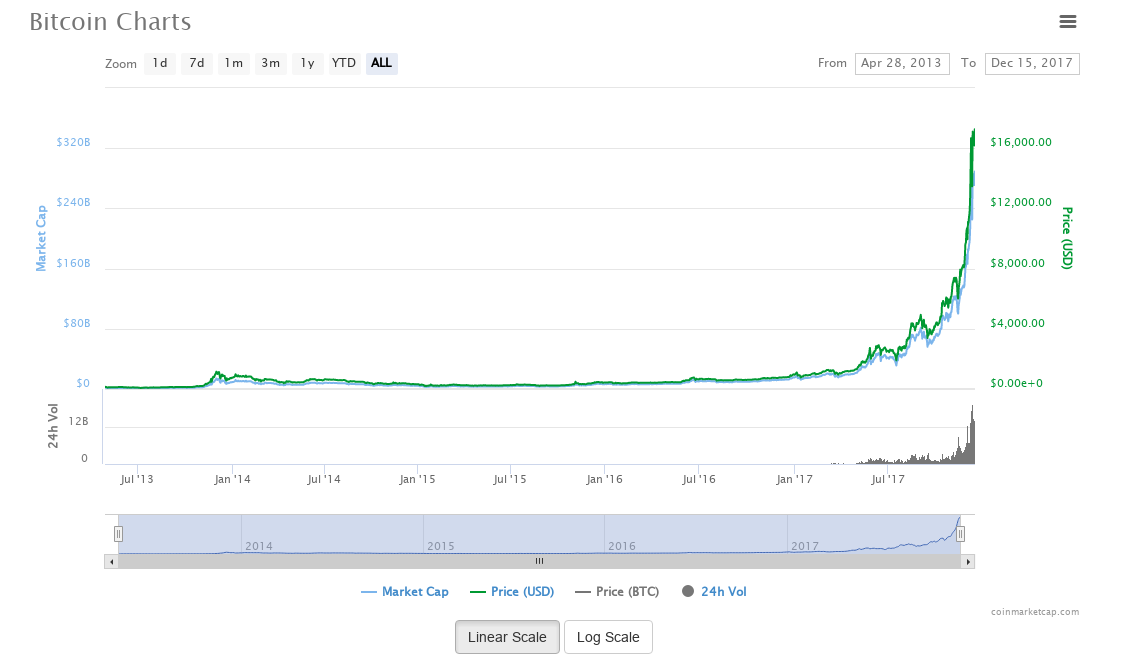
\includegraphics[scale=0.3]{bitcoin-usd-prices.png}
\end{frame}

\begin{frame}
    \frametitle{Bitcoin Mania}
    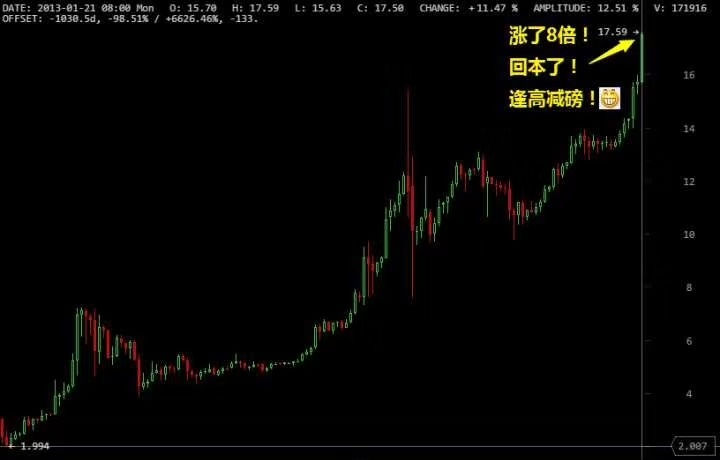
\includegraphics[scale=0.3]{bitcoin-invest0.jpg}
\end{frame}

\begin{frame}
    \frametitle{Bitcoin Mania}
    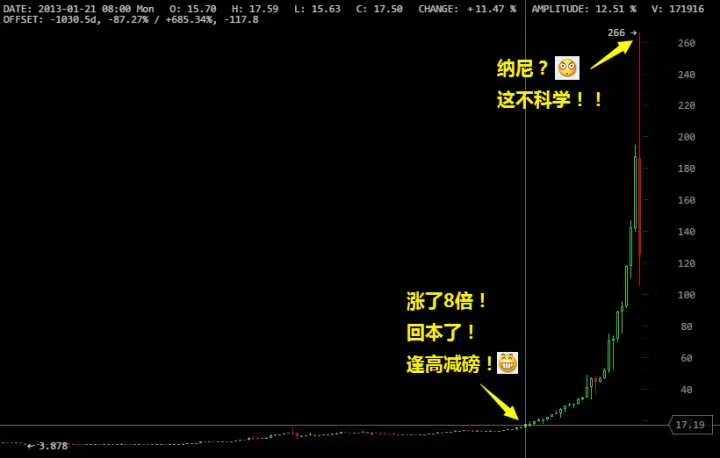
\includegraphics[scale=0.3]{bitcoin-invest1.jpg}
\end{frame}

\begin{frame}
    \frametitle{Bitcoin Mania}
    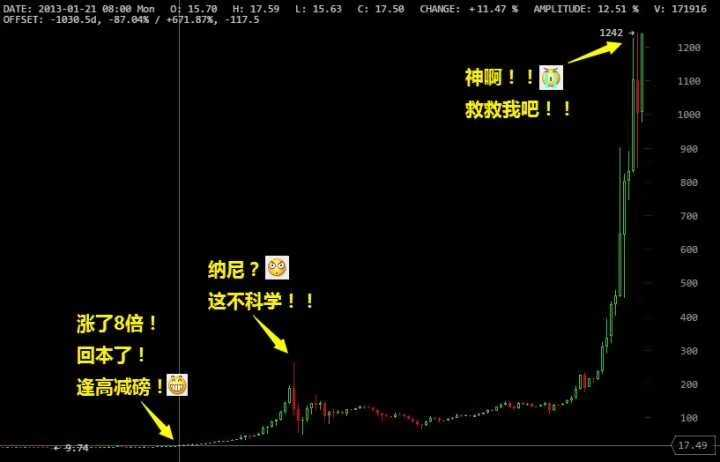
\includegraphics[scale=0.3]{bitcoin-invest2.jpg}
\end{frame}

\begin{frame}
    \frametitle{Bitcoin Mania}
    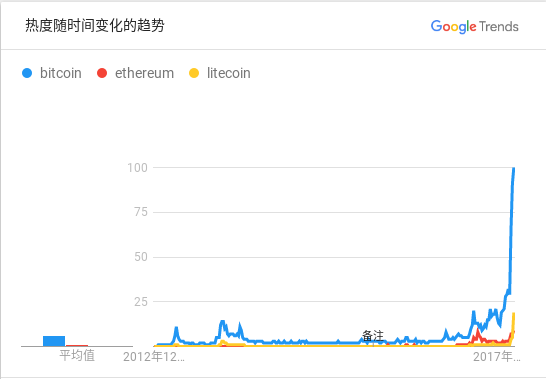
\includegraphics[scale=0.4]{bitcoin-google-trends.png}
\end{frame}

\begin{frame}
    \frametitle{Bitcoin Mania}
    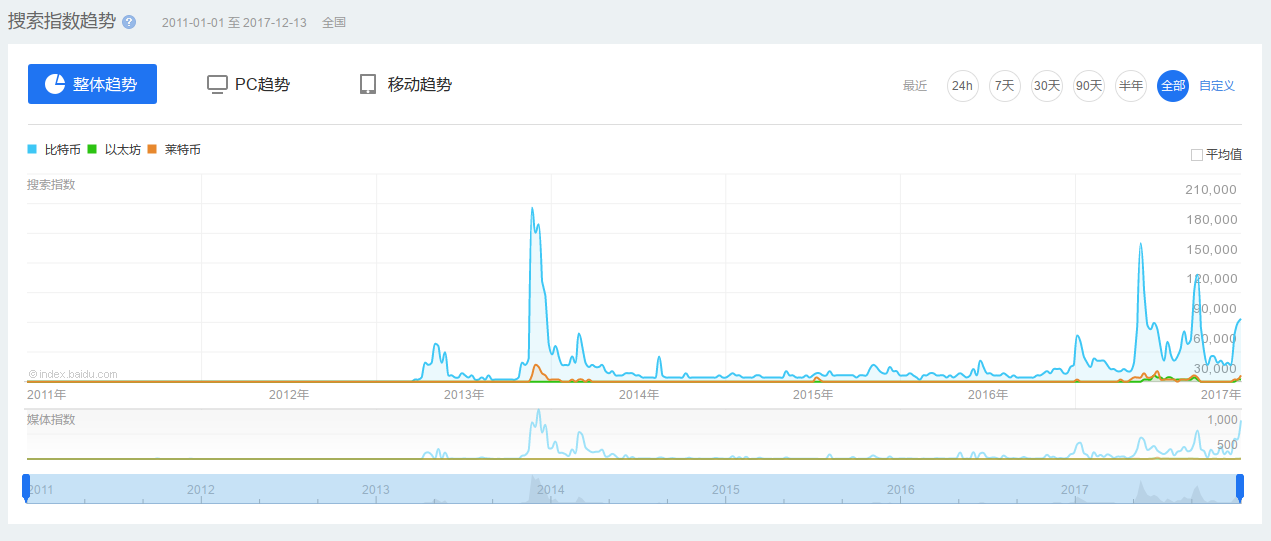
\includegraphics[scale=0.26]{bitcoin-baidu-index.png}
\end{frame}

\begin{frame}
    \frametitle{BlockChain}
    \begin{block}{国务院2016年十三五报告}
        “十三五”时期,全球信息化发展面临的环境、条件和内涵正发生深刻变化 \ldots
        信息技术创新代际周期大幅缩短,创新活力、集聚效应和应用潜能裂变式释放,更快速度、更广范围、更深程度地引发新一轮科技革命和产业变革。物联网、云计算、大数据、人工智能、机器深度学习、\alert{区块链}、生物基因工程等新技术驱动网络空间从人人互联向万物互联演进,数字化、网络化、智能化服务将无处不在。现实世界和数字世界日益交汇融合,全球治理体系面临深刻变革。全球经济体普遍把加快信息技术创新、最大程度释放数字红利,作为应对“后金融危机”时代增长不稳定性和不确定性、深化结构性改革和推动可持续发展的关键引擎。
    \end{block}
\end{frame}

\begin{frame}
    \frametitle{Barter System}
    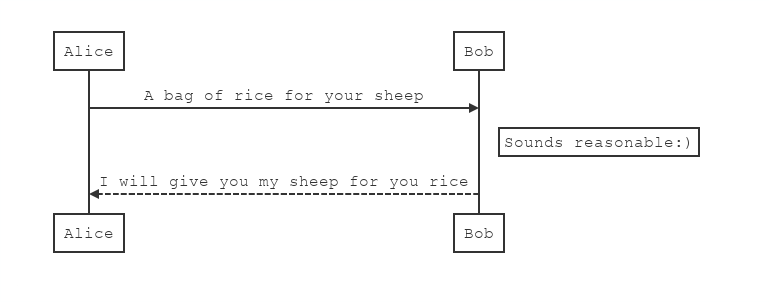
\includegraphics[scale=0.4]{barter-system.png}
\end{frame}

\begin{frame}
    \frametitle{Gold Money}
    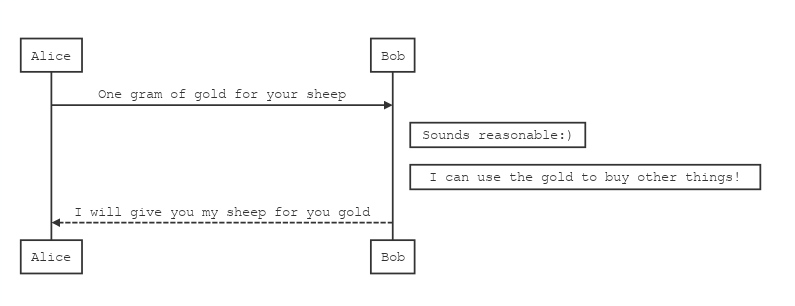
\includegraphics[scale=0.4]{gold-money.png}
\end{frame}

\begin{frame}
    \frametitle{Paper Money}
    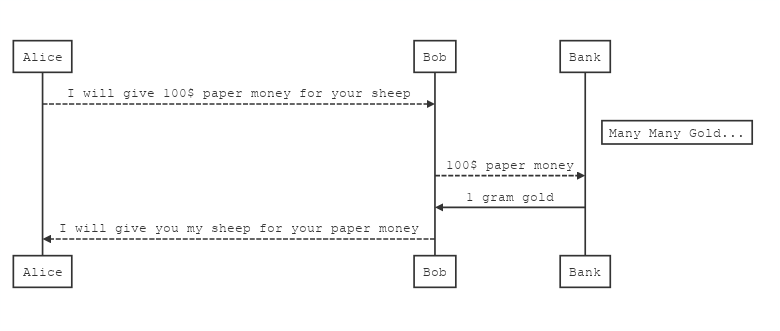
\includegraphics[scale=0.4]{paper-money.png}
\end{frame}

\begin{frame}
    \frametitle{Central Banking}
    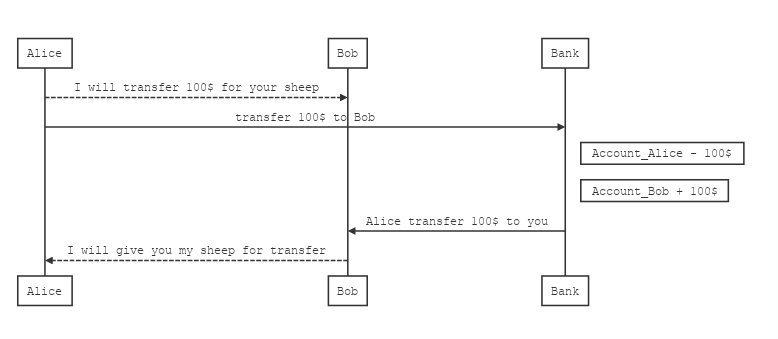
\includegraphics[scale=0.4]{central-banking.png}
\end{frame}

\begin{frame}
    \frametitle{Nature of Money}
    \textbf{What is Money?}
    \begin{itemize}
        \item \textbf{Medium of exchange}
            \begin{itemize}
                \item Standard object used in exchanging goods and services
            \end{itemize}
        \item \textbf{Unit of account}
            \begin{itemize}
                \item Standard unit used for quoting prices
            \end{itemize}
        \item \textbf{Store of value}
            \begin{itemize}
                \item Store wealth from one point in time to another
            \end{itemize}
    \end{itemize}
\end{frame}

\begin{frame}
    \frametitle{What is Bitcoin?}
    \begin{block}{Wikipedia}
        Bitcoin is the first \alert{decentralized digital cryptocurrency}, as the \alert{worldwide payment system} works without a central bank or single administrator. The network is \alert{peer-to-peer} and transactions take place between users directly through the use of cryptography, without an intermediary. These \alert{transactions} are verified by network nodes, which called \alert{mining} and recorded in a \alert{public distributed ledger} called a \alert{blockchain}. Bitcoin was invented by an unknown person or group of people under the name \alert{Satoshi Nakamoto} and released as \alert{open-source software} in 2009.
    \end{block}
\end{frame}

\begin{frame}
    \frametitle{Video}
    \begin{center}
        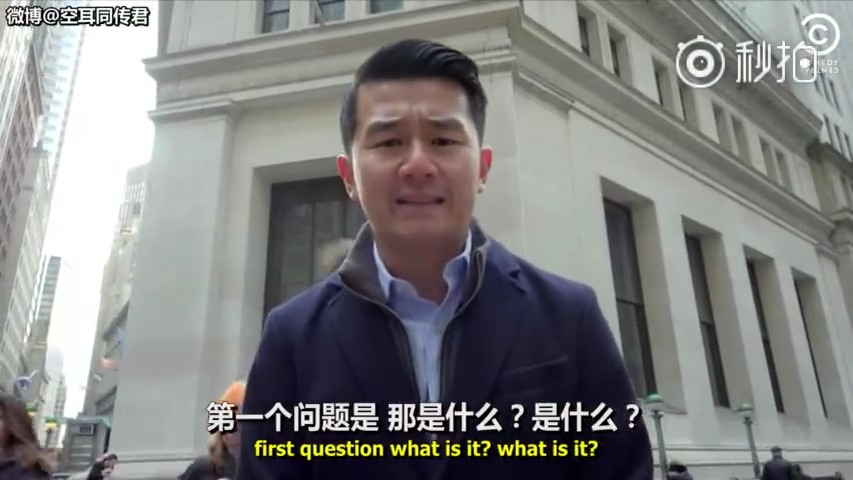
\includegraphics[scale=0.35]{what-it-it.jpg} \\
        \href{run:cryptocurrency.mp4}{\textbf{Bitcoin, What is it?}}
    \end{center}
\end{frame}

\begin{frame}
    \frametitle{Bitcoin Overview}
    
\includegraphics[scale=1]{mbc2_0201.png}
\end{frame}

\begin{frame}[fragile]
    \frametitle{Buying a cup of coffee}
    Alice buyes a cup of coffee at Bob's coffee shop, paying with BTC.
    \begin{columns}
        \begin{column}{0.6\textwidth}
            \begin{lstlisting}[language=Python]
bitcoin:1GdK9UzpHBzqzX2A9JFP3Di4weBwqgmoQA?\
amount=0.015&\
label=Bob%27s%20Cafe&\
message=Purchase%20at%20Bob%27s%20Cafe

Components of the URL
A bitcoin address: "1GdK9UzpHBzqzX2A9JFP3Di4weBwqgmoQA"
The payment amount: "0.015"
A label for the recipient address: "Bob's Cafe"
A description for the payment: "Purchase at Bob's Cafe"
            \end{lstlisting}
        \end{column}
        \begin{column}{0.3\textwidth}
            
\includegraphics[scale=1]{mbc2_0202.png}
        \end{column}
    \end{columns}
\end{frame}

\begin{frame}
    \begin{center}
        \textbf{\alert{\huge{Q \& A}}}
    \end{center}
\end{frame}

\begin{frame}
    \frametitle{Bitcoin: Challenges}
    \begin{itemize}
        \item \textbf{Creation of a virtual coin}
            \begin{itemize}
                \item How is it created in the first place?
                \item How do you prevent inflation?
            \end{itemize}
        \item \textbf{Validation}
            \begin{itemize}
                \item Is the coin legit? \alert{(Proof-Of-Work)}
                \item How do you prevent a coin from \alert{double-spending}?
            \end{itemize}
        \item \textbf{Buyer and seller protection in online transactions}
            \begin{itemize}
                \item Buyer pays, but the seller doesn't deliver
                \item Seller delivers, buyer pays, but the buyer makes a claim
            \end{itemize}
        \item \textbf{Trust on third party}
            \begin{itemize}
                \item Rely on proof instead of trust
                \item Verifiable by everyone
                \item No central bank
            \end{itemize}
    \end{itemize}
\end{frame}

\begin{frame}
    \frametitle{CryptoCurrency}
    
\includegraphics[scale=0.16]{cryptocurrency.png}
\end{frame}

\begin{frame}[fragile]
    \frametitle{Bitcoin Overview}
    \begin{lstlisting}[language=JavaScript]
function mine()
{
    while (true)
    {
        longestChain = getLongestValidChain();

         A number that changes every time, so that you don't waste time
         trying to calculate a valid blockHash with the same input.
        nonce = getNewNonce();

        currentTXs = getUnconfirmedTransactionsFromNetwork();
        newBlock = getNewBlock(longestChain, currentTX, nonce);

         Hash function, and this is what all the *mining machines* are doing
        blockHash = sha256(newBlock)

        if (meetRequirements(blockHash))
        {
            broadcast(newBlock)
             now the height of the block chain is incremented by 1
             if the new block is accepted by other peers
             and all the TXs in the new block are "confirmed"
        }
    }
}
    \end{lstlisting}
\end{frame}

\begin{frame}[fragile]
    \frametitle{Bitcoin Overview}
    \begin{lstlisting}[language=JavaScript]
function sendBTC(amount)
{
    sourceTXs = pickConfirmedTransactionsToBeSpent(amount);
    tx = generateTX(sourceTx, targetAddrs, amount, fee);
    signedTx = sign(tx, privateKeysOfAllInputAddress);
    broadcast(signedTx);
}
    \end{lstlisting}
\end{frame}



\section{P2P Network}
\begin{frame}
    \frametitle{P2P Network}
    The steps to run the network are as follows:
    \begin{itemize}
        \item New transactions are broadcast to all nodes.
        \item Each node collects new transactions into a block.
        \item When node finds a proof-of-work, it broadcast the block to all nodes.
        \item Nodes accept the block only if all transactions in it are valid and not already spent.
        \item Nodes express their acceptance of the block by working on creating the next block in the chain, using the hash of the accepted block as previous hash.
    \end{itemize}
\end{frame}

\begin{frame}
    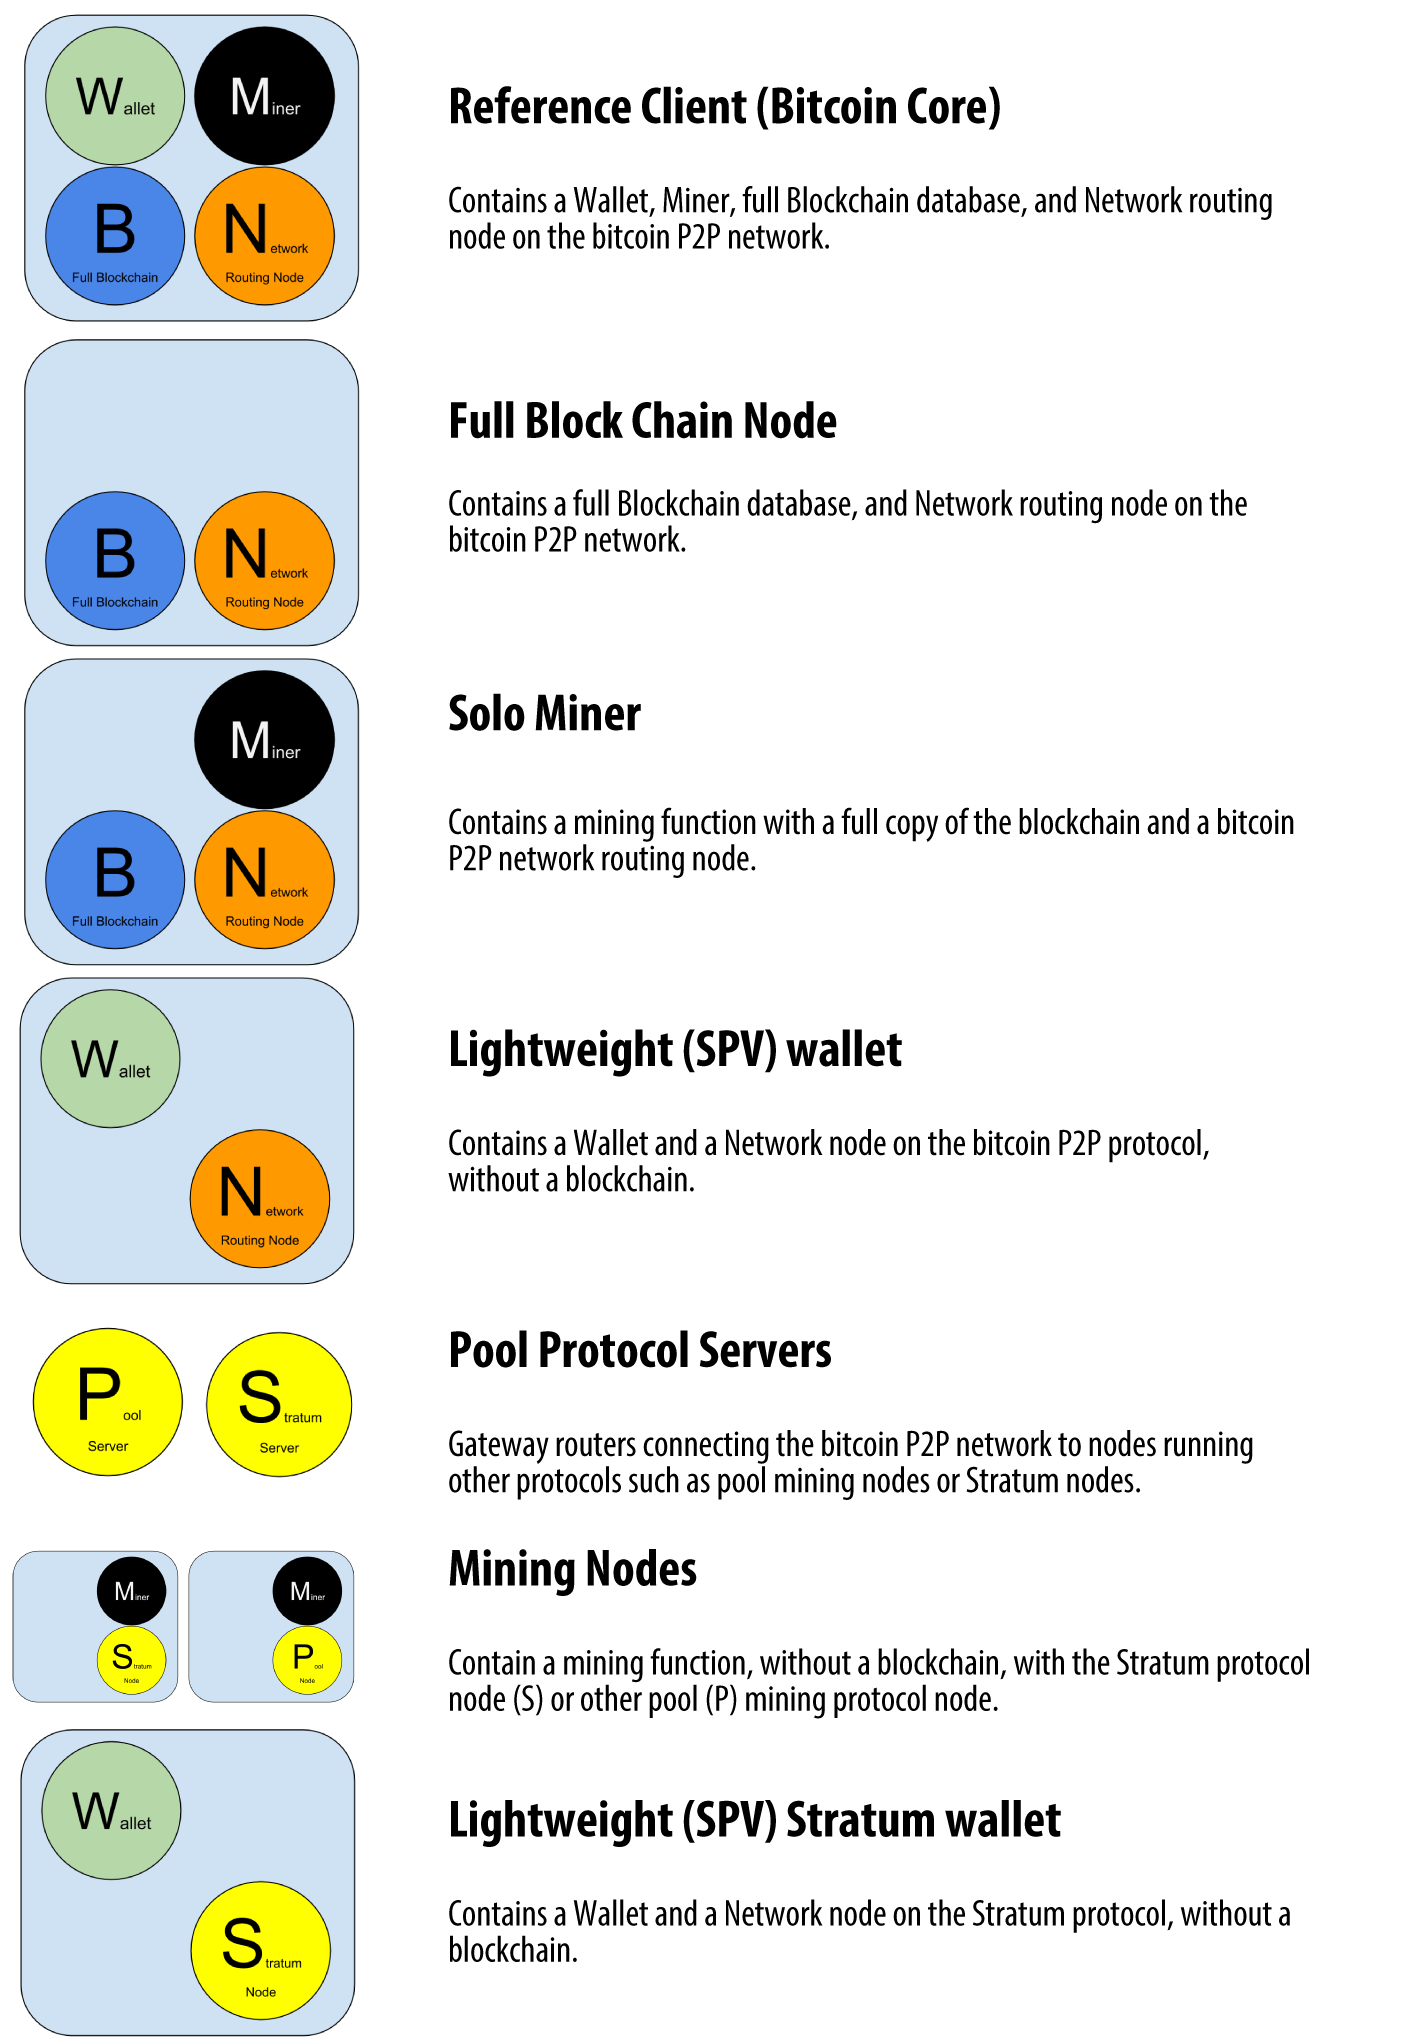
\includegraphics[scale=0.6]{./figures/mbc2_0802.png}
\end{frame}

\begin{frame}
    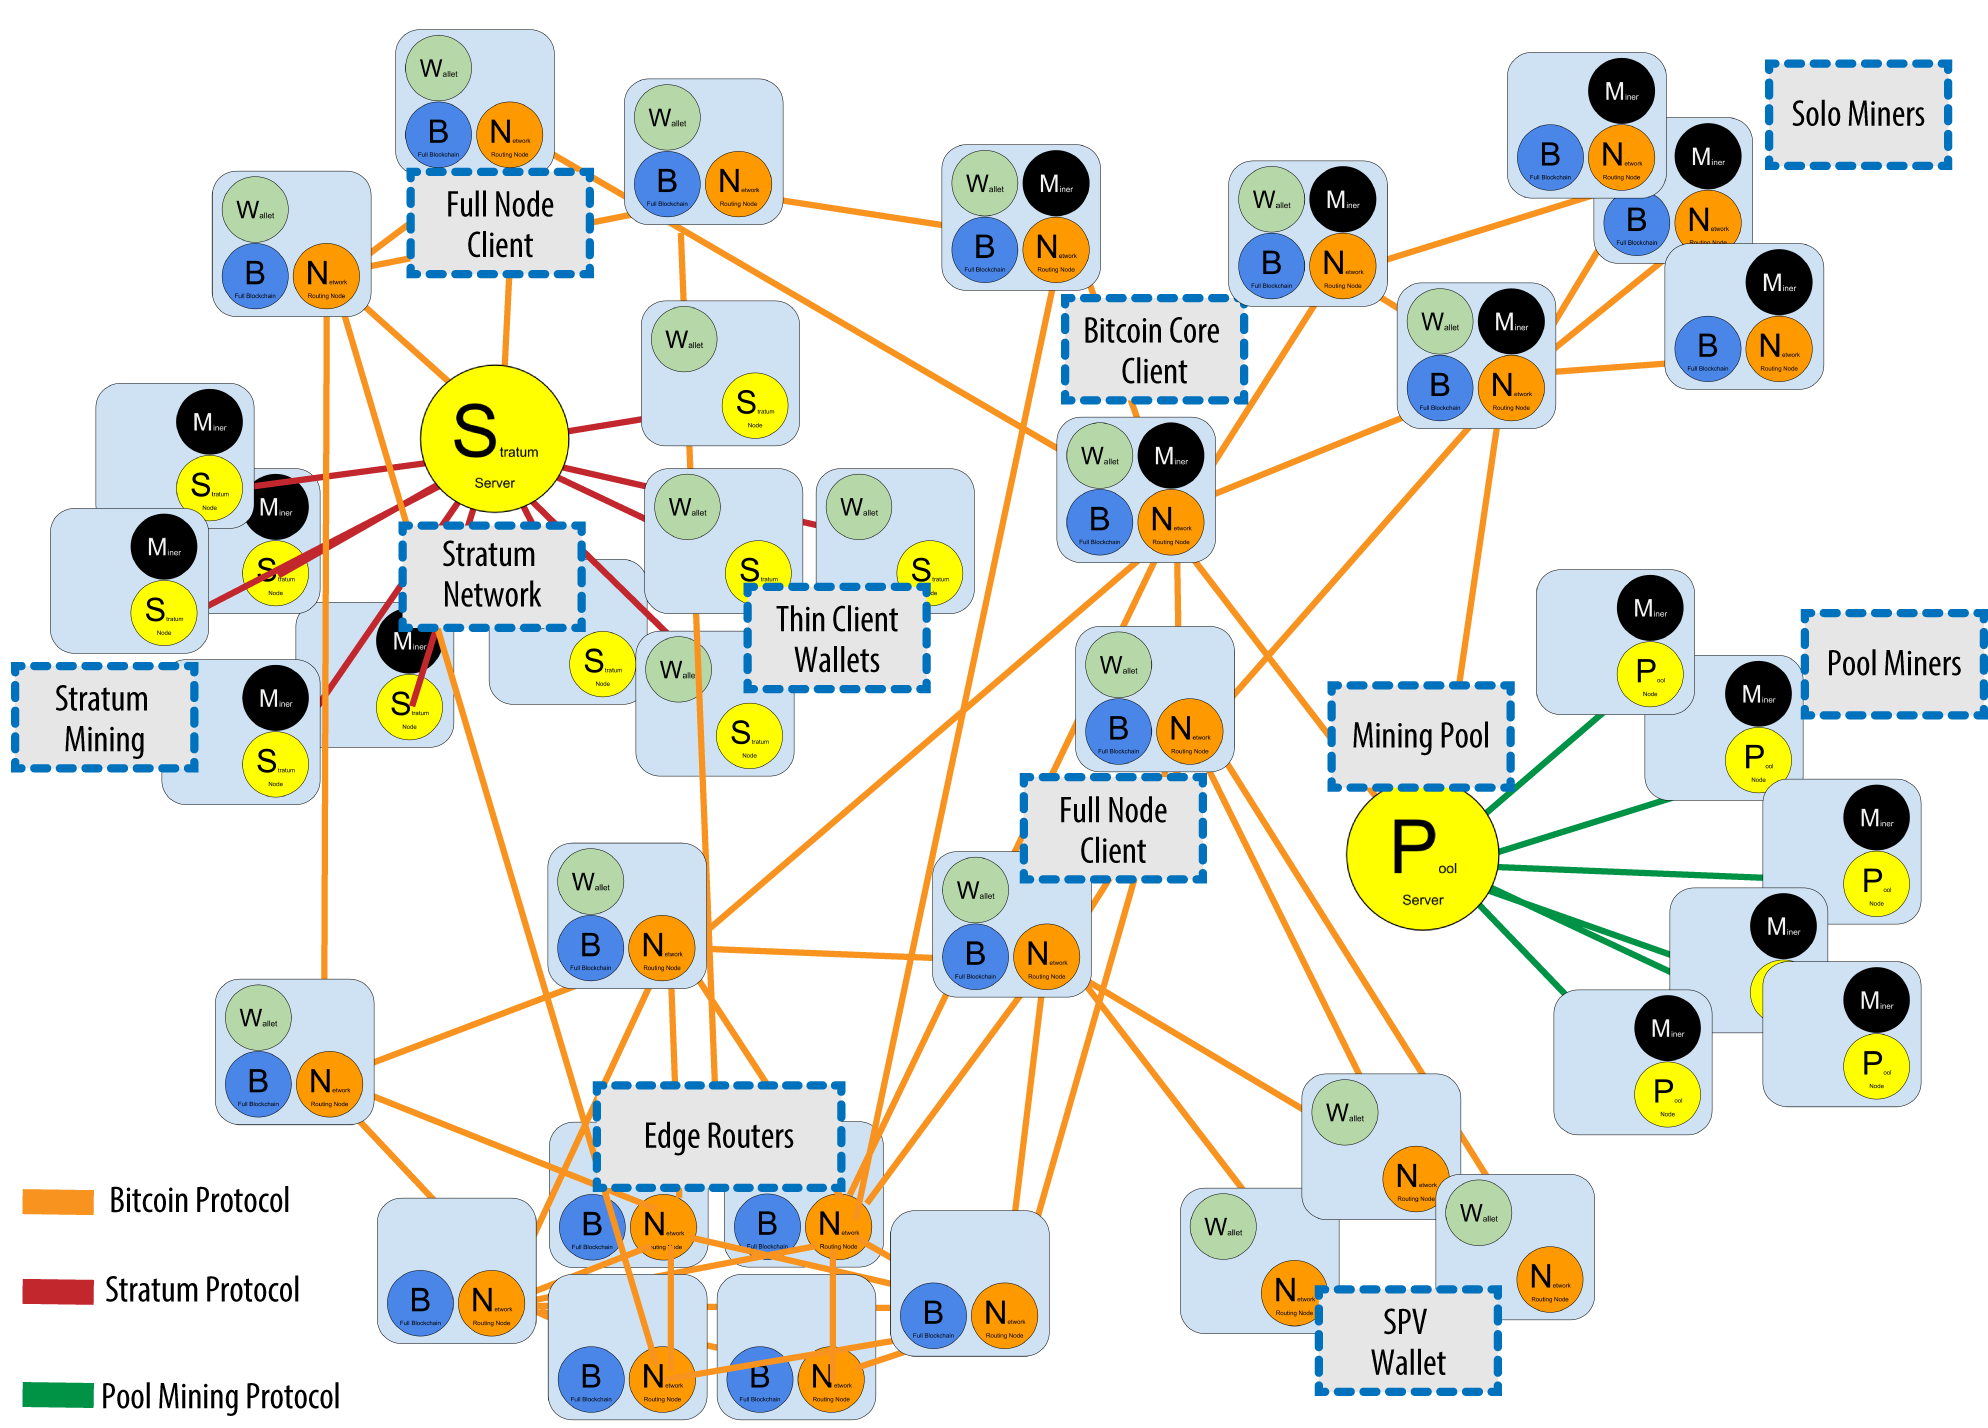
\includegraphics[scale=0.15]{./figures/mbc2_0803.png}
\end{frame}


\section{Crypto}
\begin{frame}
    \frametitle{Security in Bitcoin}
    \begin{itemize}
        \item \textbf{Authentication}
            \begin{itemize}
                \item Am I paying the right person?
            \end{itemize}
        \item \textbf{Integrity}
            \begin{itemize}
                \item Is the coin double-spent?
                \item Can an attacker reverse or change transactions?
            \end{itemize}
        \item \textbf{Availability}
            \begin{itemize}
                \item Can I make a transactions anytime I want?
            \end{itemize}
        \item \textbf{Confidentiality}
            \begin{itemize}
                \item Are my transactions private? Anonymous?
            \end{itemize}
    \end{itemize}
\end{frame}

\begin{frame}
    \frametitle{Security in Bitcoin}
    \begin{itemize}
        \item \textbf{Authentication -> \alert{Public Key Crypto: Digital Signatures}}
            \begin{itemize}
                \item Am I paying the right person?
            \end{itemize}
        \item \textbf{Integrity -> \alert{Digital Signatures and Cryptographic Hash}}
            \begin{itemize}
                \item Is the coin double-spent?
                \item Can an attacker reverse or change transactions?
            \end{itemize}
        \item \textbf{Availability -> \alert{Broadcast messages to the P2P network}}
            \begin{itemize}
                \item Can I make a transactions anytime I want?
            \end{itemize}
        \item \textbf{Confidentiality -> \alert{Pesudonymity}}
            \begin{itemize}
                \item Are my transactions private? Anonymous?
            \end{itemize}
    \end{itemize}
\end{frame}

\begin{frame}
    \frametitle{Cryptographic Hash Function}
    \begin{itemize}
        \item \textbf{Computationally efficient}
        \item \textbf{Consistent} \\
            hash(x) always yields same result.
        \item \textbf{Collision Resistant} \\
            Given $hash(W) = Z$, hard to find X such that $hash(X) = Z$
        \item \textbf{One-way} \\
            Given Y, hard to find X s.t. $hash(X) = Y$
    \end{itemize}
    \begin{columns}
        \begin{column}{0.5\textwidth}
            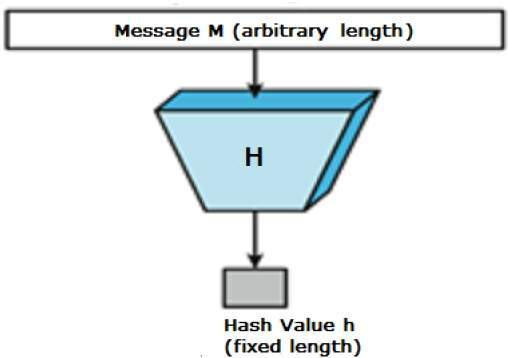
\includegraphics[scale=0.3]{hash_functions.jpg}
        \end{column}
        \begin{column}{0.5\textwidth}
            Common Hash Functions:
            \begin{itemize}
                \item \textbf{MD5}
                \item \textbf{SHA-1}
                \item \textbf{SHA-2}
                    \begin{itemize}
                        \item SHA-256
                        \item SHA-384
                        \item SHA-512
                    \end{itemize}
            \end{itemize}
        \end{column}
    \end{columns}
\end{frame}

\begin{frame}[fragile]
    \frametitle{Hash Function Example}
    \begin{lstlisting}[language=Python]
    SHA224("")
    0x d14a028c2a3a2bc9476102bb288234c415a2b01f828ea62ac5b3e42f
    SHA256("")
    0x e3b0c44298fc1c149afbf4c8996fb92427ae41e4649b934ca495991b7852b855
    \end{lstlisting}

    Even a small change in the message wil result in a mostly different hash.
    \begin{lstlisting}[language=Python]
    SHA224("The quick brown fox jumps over the lazy dog")
    0x 730e109bd7a8a32b1cb9d9a09aa2325d2430587ddbc0c38bad911525
    SHA224("The quick brown fox jumps over the lazy dog.")
    0x 619cba8e8e05826e9b8c519c0a5c68f4fb653e8a3d8aa04bb2c8cd4c
    \end{lstlisting}

    Proof of work first sight:

    Given a basic string \alert{hello world!} + random number \alert{nonce}

    We need the digest have 4 leading 0.
    \begin{lstlisting}[language=Python]
    "Hello, world!0" => 1312af178c253f84028d480a6adc1e25e81caa44c749ec81976192e2ec934c64
    "Hello, world!1" => e9afc424b79e4f6ab42d99c81156d3a17228d6e1eef4139be78e948a9332a7d8
    "Hello, world!2" => ae37343a357a8297591625e7134cbea22f5928be8ca2a32aa475cf05fd4266b7
    ...
    "Hello, world!4248" => 6e110d98b388e77e9c6f042ac6b497cec46660deef75a55ebc7cfdf65cc0b965
    "Hello, world!4249" => c004190b822f1669cac8dc37e761cb73652e7832fb814565702245cf26ebb9e6
    "Hello, world!4250" => 0000c3af42fc31103f1fdc0151fa747ff87349a4714df7cc52ea464e12dcd4e9
    \end{lstlisting}
\end{frame}

\begin{frame}
    \frametitle{Public Key Crypto: Encryption}
    Key pair: Public Key and Private Key
    \begin{columns}
        \begin{column}{0.35\textwidth}
            \begin{center}
                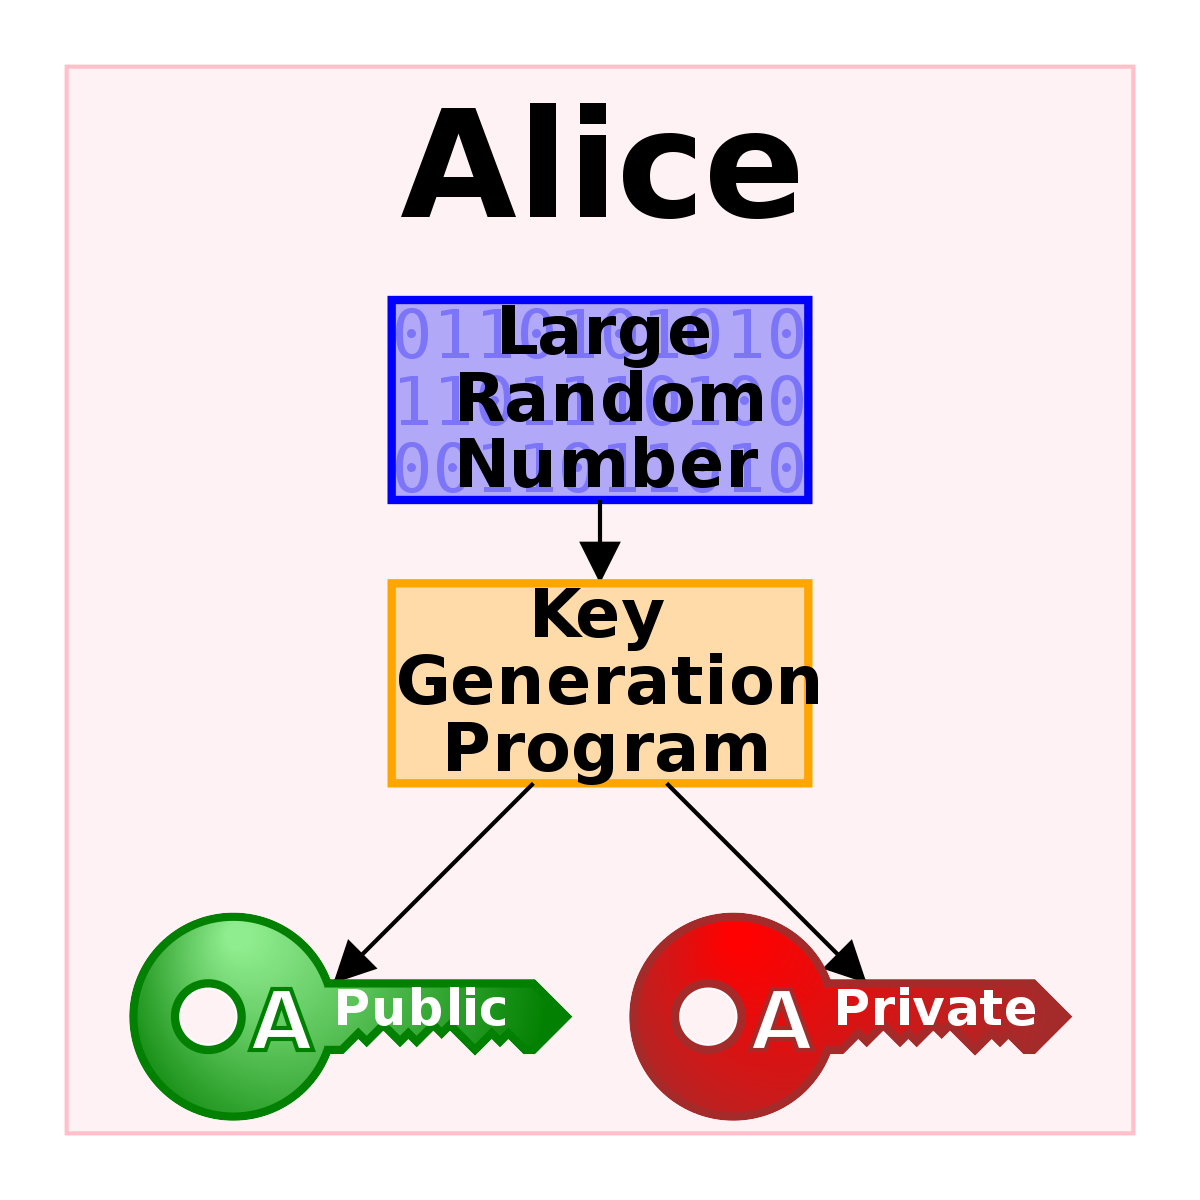
\includegraphics[scale=0.1]{Public-key-crypto.png}
            \end{center}
        \end{column}
        \begin{column}{0.65\textwidth}
            \begin{center}
                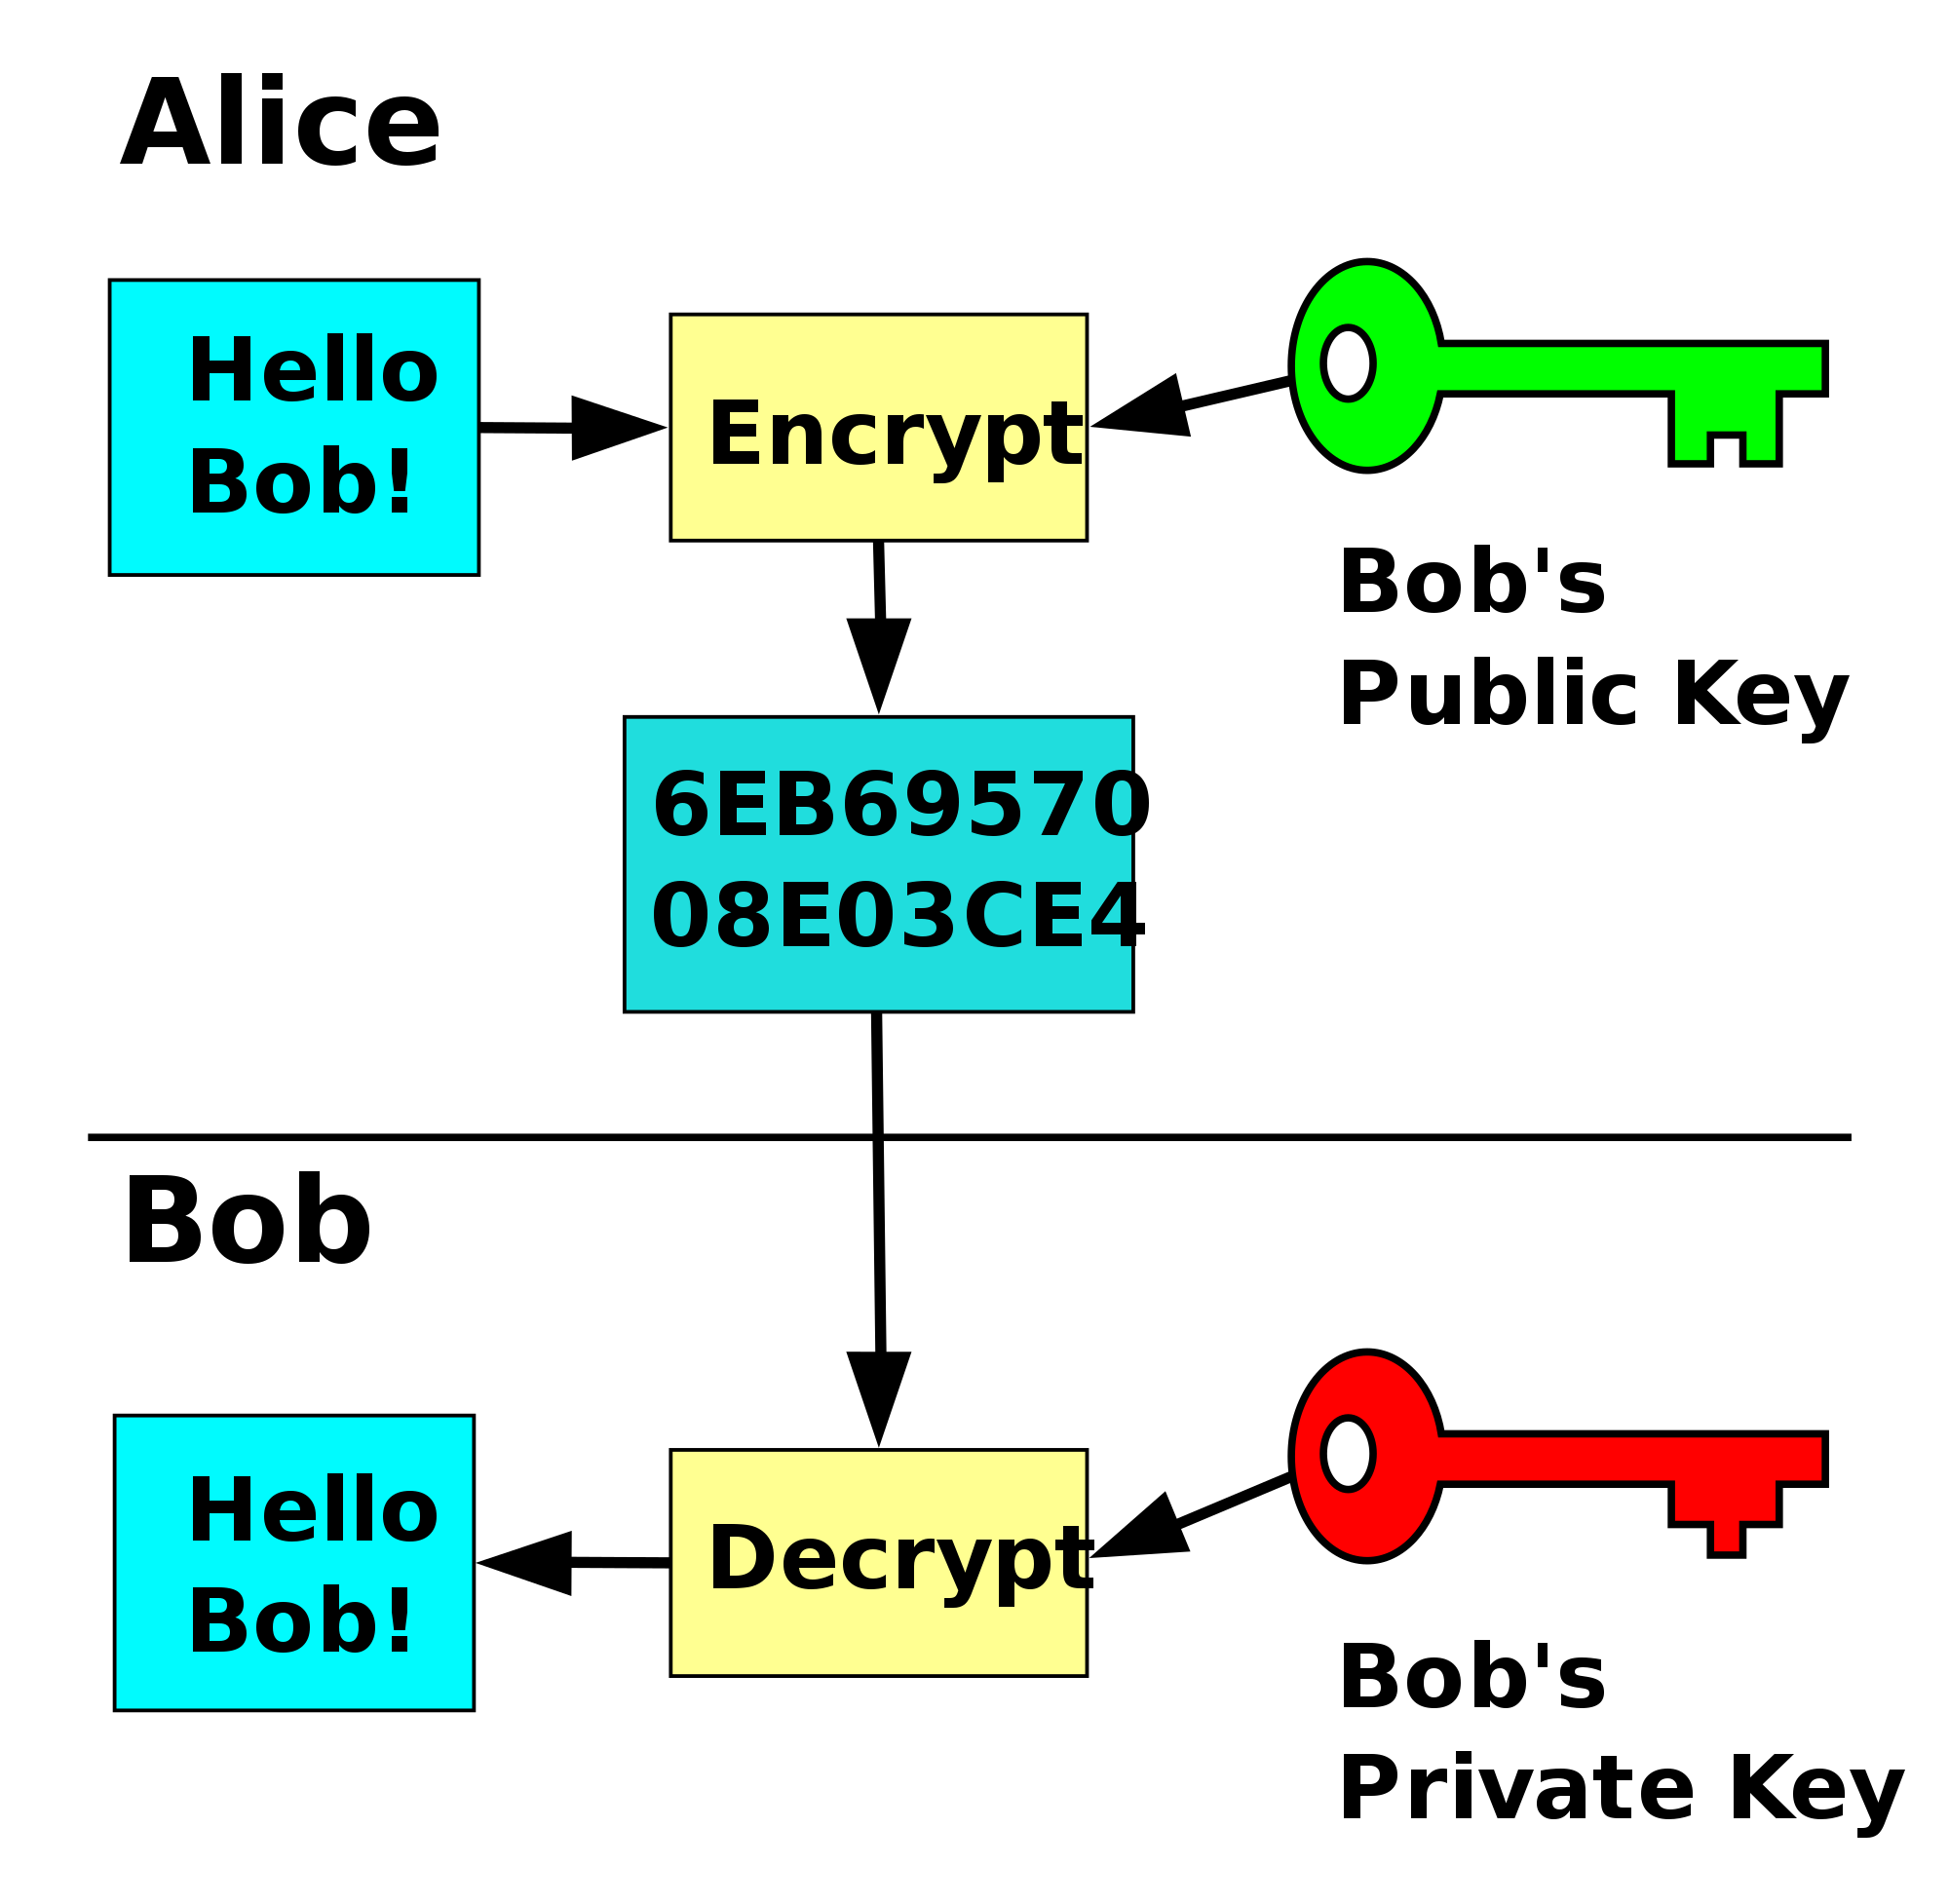
\includegraphics[scale=0.1]{Public_key_shared_secret.png}
            \end{center}
        \end{column}
    \end{columns}
\end{frame}

\begin{frame}
    \frametitle{Public Key Crypto: Digital Signature}
    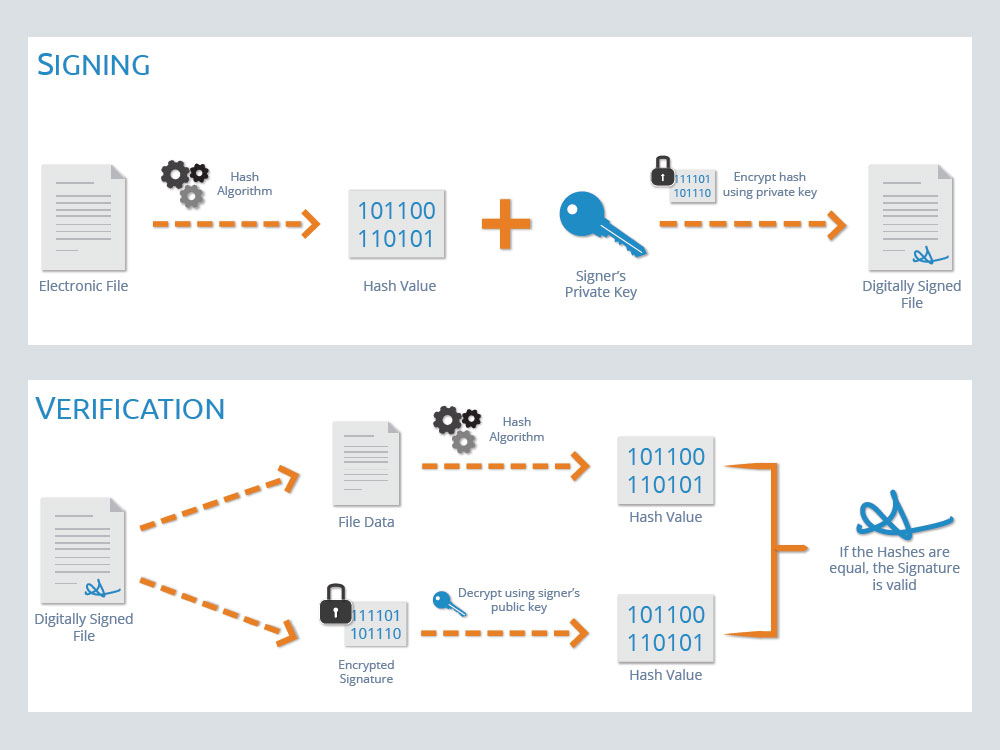
\includegraphics[scale=0.3]{digital-signatures-methodology.jpg}
\end{frame}

\begin{frame}
    \frametitle{Public Key to Bitcoin Address}
    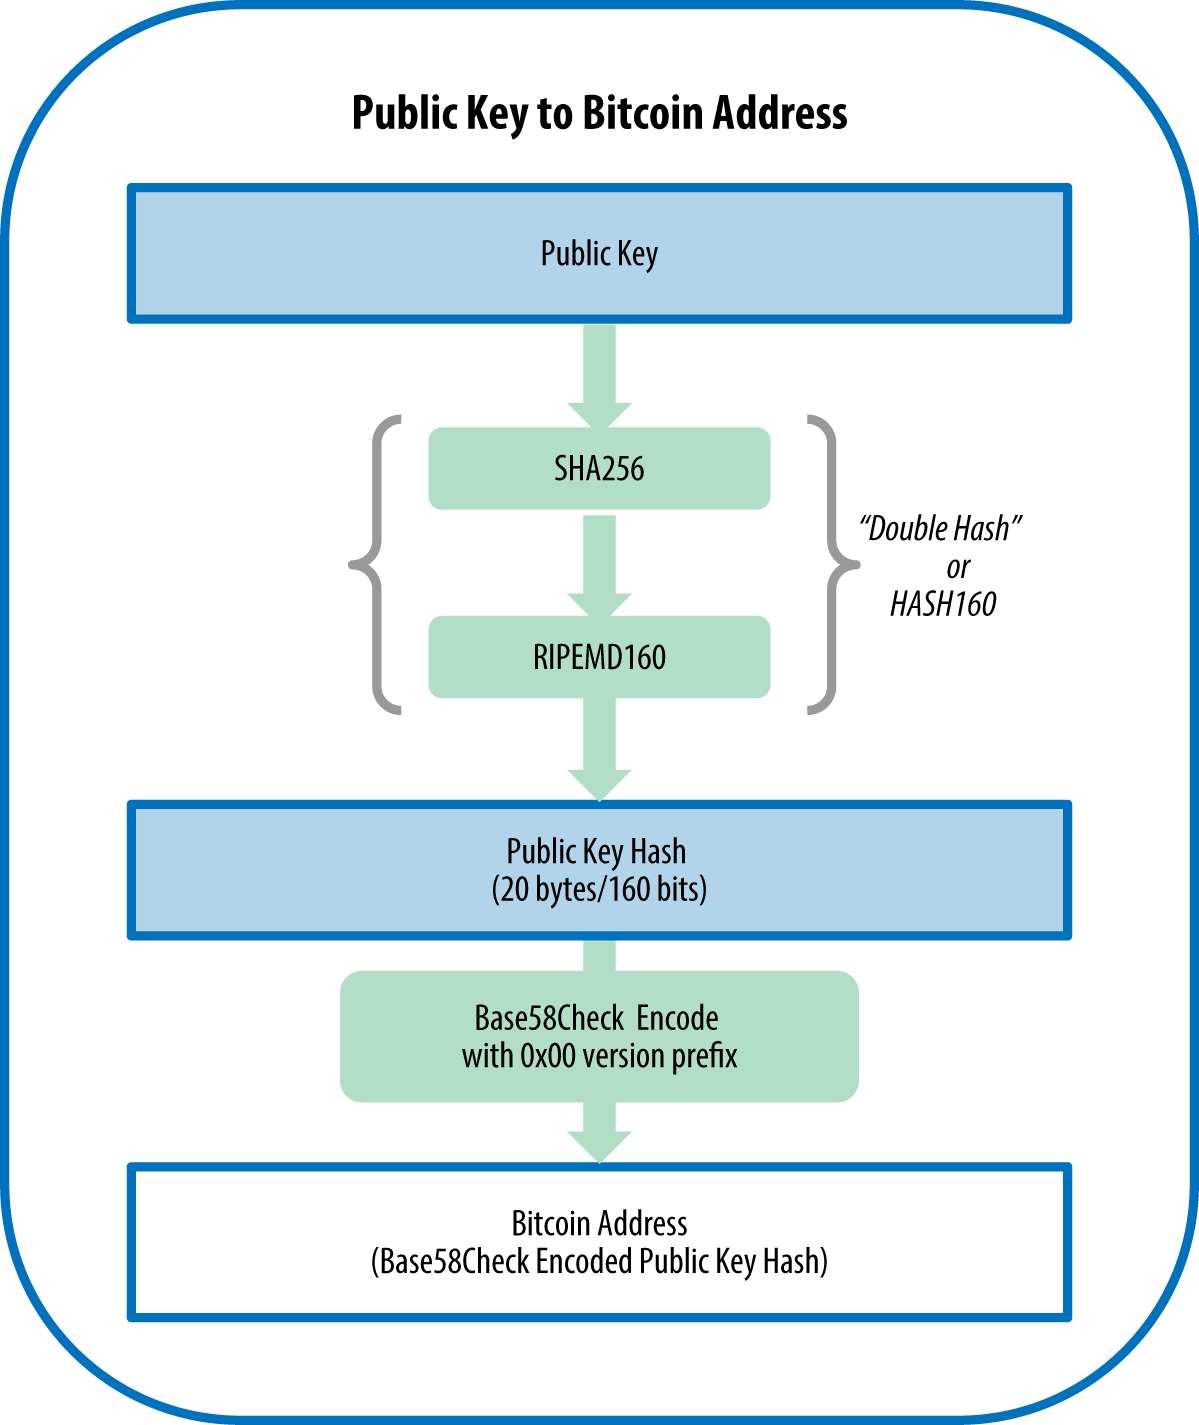
\includegraphics[scale=0.5]{mbc2_0405.png}
\end{frame}



\section{Transaction}
\begin{frame}

\end{frame}


\section{BlockChain}
\begin{frame}
    \frametitle{BlockChain Overview}
    \begin{itemize}
        \item The block chain provides Bitcoin's public ledger, an ordered and timestamped record of transctions.
        \item This system is used to protect against double spending and modification of previous transactions records.
        \item Each full node in the Bitcoin network independently stores a block chain containing only blocks validated by that node.
    \end{itemize}
    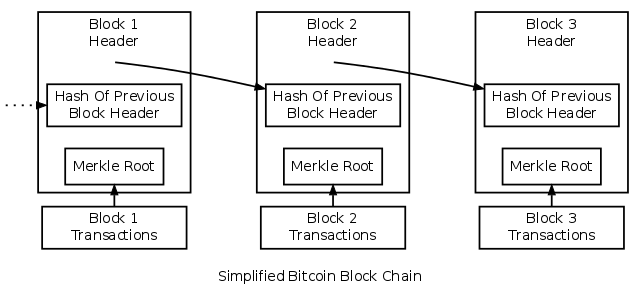
\includegraphics[scale=0.4]{./figures/en-blockchain-overview.png}
\end{frame}

\begin{frame}[fragile]
    \frametitle{BlockChain Data Structure}
    \begin{columns}
        \begin{column}{0.6\textwidth}
            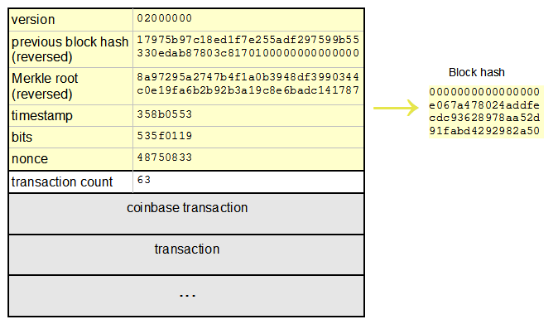
\includegraphics[scale=0.5]{./figures/blockchain-data-structure.png}
        \end{column}
        \begin{column}{0.4\textwidth}
            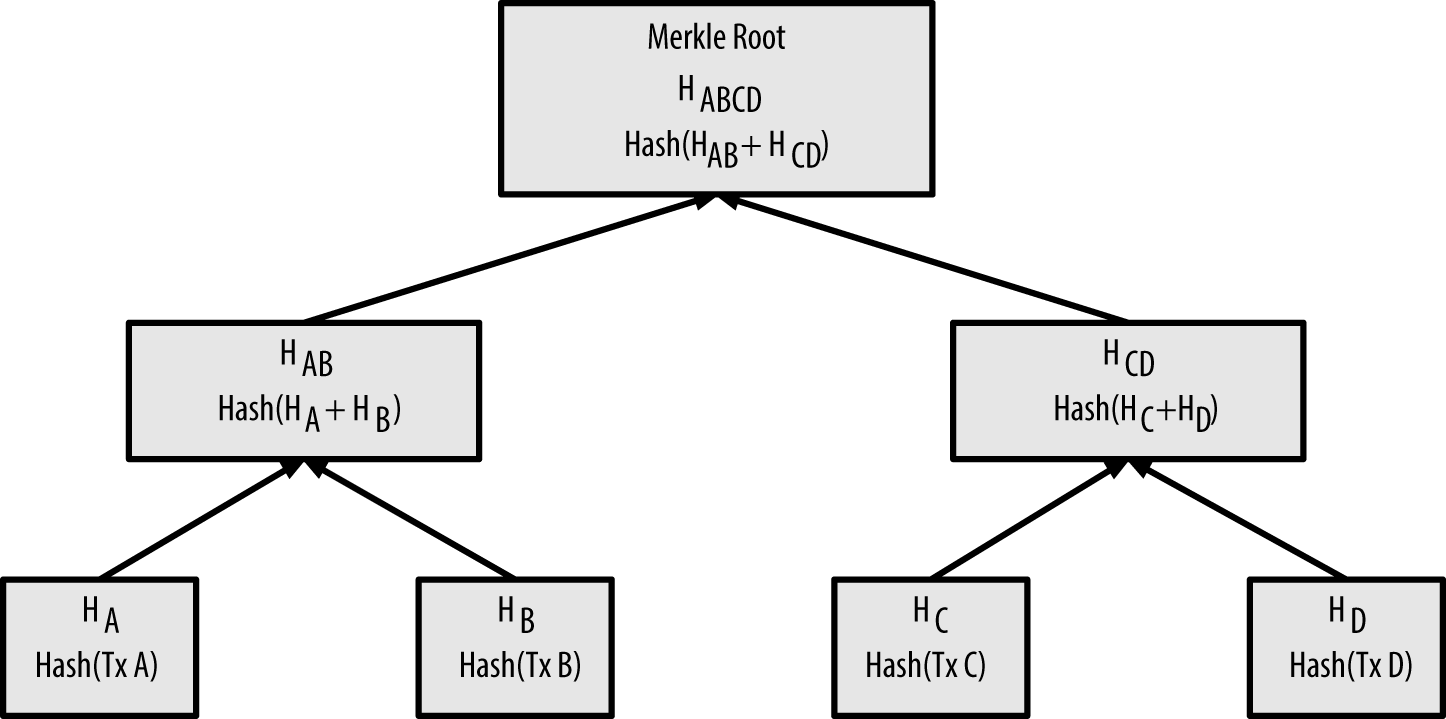
\includegraphics[scale=0.4]{./figures/mbc2_0902.png}
        \end{column}
    \end{columns}
    \begin{itemize}
        \item \textbf{Block Header}: 80 bytes, whereas transctions is at least 250 bytes.
        \item \textbf{Nonce}: A counter used for proof-of-work algorithm.
        \item \textbf{Difficulty}: How difficult it is to find a hash below a given target.
        \item \textbf{Coinbase}: The content of the \alert{input} of a generation transction.
    \end{itemize}
    \begin{lstlisting}[language=Python]
The Times 03/Jan/2009 Chancellor on brink of second bailout for banks. \end{lstlisting}
\end{frame}

\begin{frame}[fragile]
    \frametitle{The Genesis Block}
    \begin{lstlisting}[language=Python]
bitcoind getblock 000000000019d6689c085ae165831e934ff763ae46a2a6c172b3f1b60a8ce26f
{
    "hash" : "000000000019d6689c085ae165831e934ff763ae46a2a6c172b3f1b60a8ce26f",
    "confirmations" : 308321,
    "size" : 285,
    "height" : 0,
    "version" : 1,
    "merkleroot" : "4a5e1e4baab89f3a32518a88c31bc87f618f76673e2cc77ab2127b7afdeda33b",
    "tx" : [
        "4a5e1e4baab89f3a32518a88c31bc87f618f76673e2cc77ab2127b7afdeda33b"
    ],
    "time" : 1231006505,
    "nonce" : 2083236893,
    "bits" : "1d00ffff",
    "difficulty" : 1.00000000,
    "nextblockhash" : "00000000839a8e6886ab5951d76f411475428afc90947ee320161bbf18eb6048"
}
    \end{lstlisting}
    The difficulty value updates every 2 weeks to ensure that it takes 10 minutes(on average) to add a new block to the BlockChain.
    \begin{lstlisting}[language=Python]
0x00ffff * 2**(8*(0x1d-3))=0x00000000FFFF0000000000000000000000000000000000000000000000000000 \end{lstlisting}
\end{frame}

\begin{frame}[fragile]
    \frametitle{Proof Of Work}
    \begin{itemize}
        \item Block contains transctions to be validated and previous hash value.
        \item Pick a nonce such that \textbf{H(prev hash, nonce, Tx) < E}.
        \item Verification is easy, But proof-of-work is hard.
    \end{itemize}
    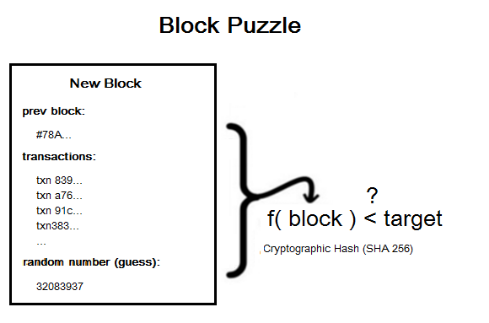
\includegraphics[scale=0.5]{./figures/block-puzzle.png}
\end{frame}

\begin{frame}[fragile]
    \frametitle{Difficulty Target and Re-Target}
    Every 2016 blocks, all node re-target the Proof-of-Work difficulty.
    \begin{lstlisting}[language=Python]
New Difficulty = Old Difficulty * (20160 minutes / Actual Time of Last 2016 Blocks)
The Target = The maximum target / current difficulty.
The maximum target is:
    0x00000000FFFF0000000000000000000000000000000000000000000000000000 \end{lstlisting}

    Re-Target Code in bitcoind
    \begin{lstlisting}[language=C++]
    // Limit adjustment step
    int64_t nActualTimespan = pindexLast->GetBlockTime() - nFirstBlockTime;
    LogPrintf("  nActualTimespan = %d  before bounds\n", nActualTimespan);
    if (nActualTimespan < params.nPowTargetTimespan/4)
        nActualTimespan = params.nPowTargetTimespan/4;
    if (nActualTimespan > params.nPowTargetTimespan*4)
        nActualTimespan = params.nPowTargetTimespan*4;

    // Retarget
    const arith_uint256 bnPowLimit = UintToArith256(params.powLimit);
    arith_uint256 bnNew;
    arith_uint256 bnOld;
    bnNew.SetCompact(pindexLast->nBits);
    bnOld = bnNew;
    bnNew *= nActualTimespan;
    bnNew /= params.nPowTargetTimespan;

    if (bnNew > bnPowLimit)
        bnNew = bnPowLimit; \end{lstlisting}
\end{frame}


\section{Mining}
\begin{frame}
    \frametitle{Mining and Consensus}
    \begin{block}{Definition}
        Mining \alert{secures} the bitcoin system and enables the emergence of network-wide \alert{consensus} without a \alert{central authority}. The reward of newly mined coins and transaction fees is an \alert{incentive scheme} that aligns the actions of miners with the \alert{security of the network}, while simultaneously implementing the \alert{monetary supply}.
    \end{block}
    \begin{figure}[htbp]
        \subfigure{
        \begin{minipage}[b]{0.45\textwidth}
            \centering
            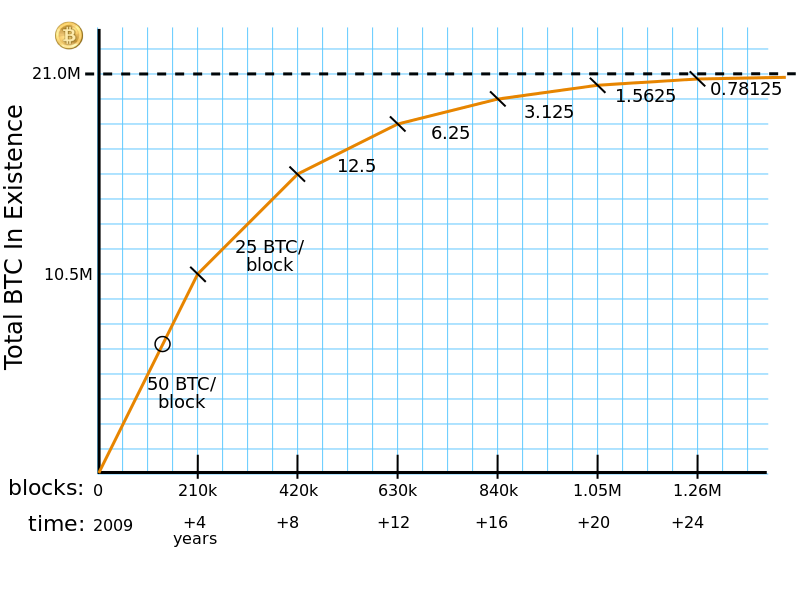
\includegraphics[scale=0.2]{mining-reward.png}
        \end{minipage}
    }
        \subfigure{
        \begin{minipage}[b]{0.45\textwidth}
            \centering
            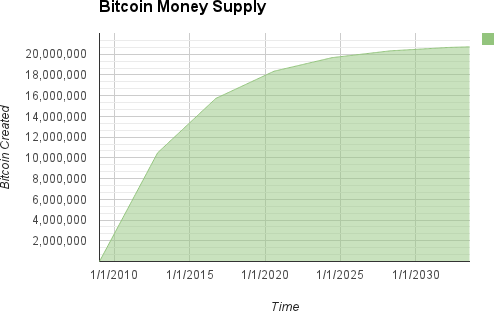
\includegraphics[scale=0.6]{mbc2_1001.png}
        \end{minipage}
    }
    \end{figure}
\end{frame}

\begin{frame}
    \frametitle{Decentralize Consensus}
    When there is no central authority, how can everyone in the network realize consensus?
    \begin{itemize}
        \item \textbf{tradition consensus algorithm}
            \begin{itemize}
                \item Paxos, Raft, \ldots
                \item Failure model: Not Byzantine(Node may fail, But not malicious)
                \item Leader election.
                \item Focusing on log(database), more universe
            \end{itemize}
        \item \textbf{blockchain consensus algorithm}
            \begin{itemize}
                \item PoW, PoS(Proof of Stake), \ldots
                \item Failure model: Byzantine(Node may be malicious)
                \item No election.
                \item Focusing on transaction.
            \end{itemize}
    \end{itemize}
    Anyway, all the consensus algorithm comply with the \alert{majority rule}.
\end{frame}

\begin{frame}
    \frametitle{Byzantine Generals' Problem}
    Story background:
    \begin{itemize}
        \item Generals of army surround enemy city
        \item Actions in union required to win
        \item Some generals may be traitors
        \item Messengers are reliable
    \end{itemize}
    \begin{center}
        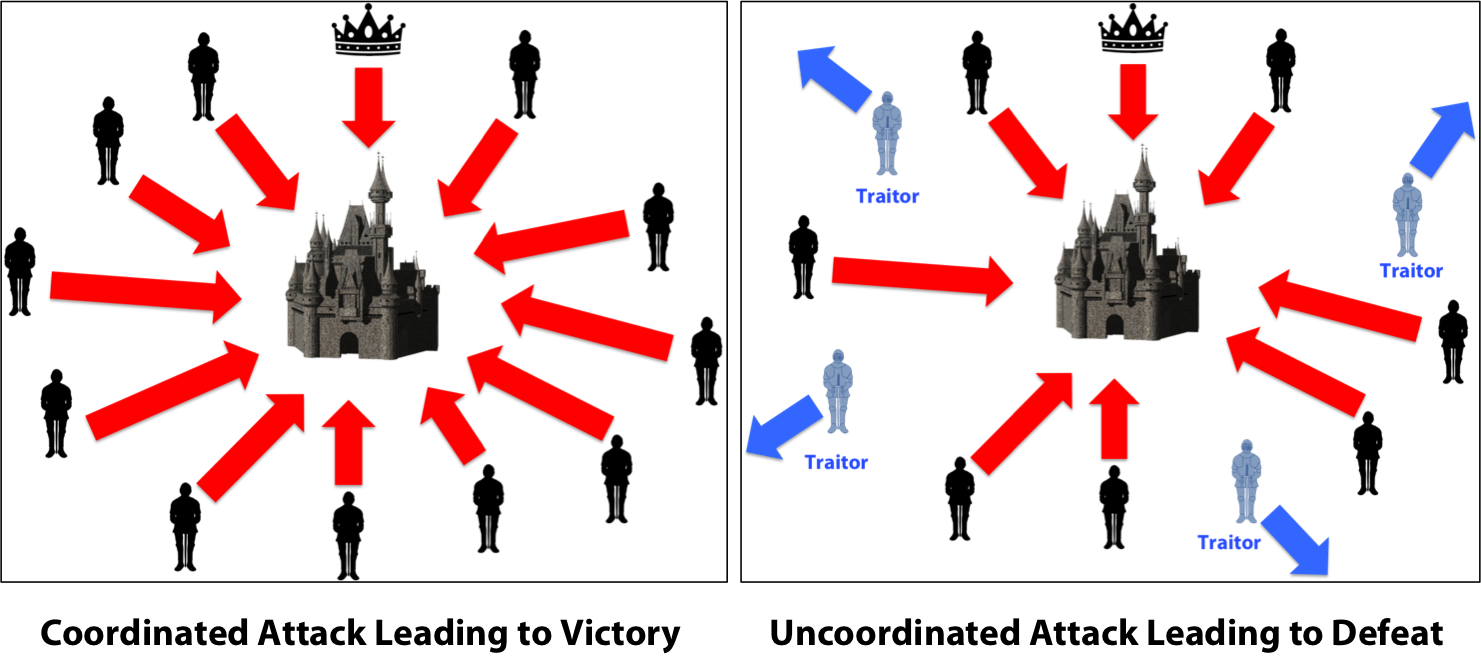
\includegraphics[scale=0.15]{byzantine-generals-problem.png}
    \end{center}
%    Results:
%    \begin{itemize}
%        \item No solution exists if less than or equal to 2/3 generals are loyal.
%    \end{itemize}
\end{frame}

\begin{frame}
    \frametitle{Proof of Work}
    \begin{itemize}
        \item \textbf{Fork}
            \begin{itemize}
                \item when 2 miners mine a block at the same time.
            \end{itemize}
        \item \textbf{Orphan}
            \begin{itemize}
                \item Only one can be in the chain, the other is called \alert{Orphan}
            \end{itemize}
        \item \textbf{Fork/Dispute Resolution}
            \begin{itemize}
                \item The longest block chain is valid.
            \end{itemize}
    \end{itemize}
    \begin{center}
        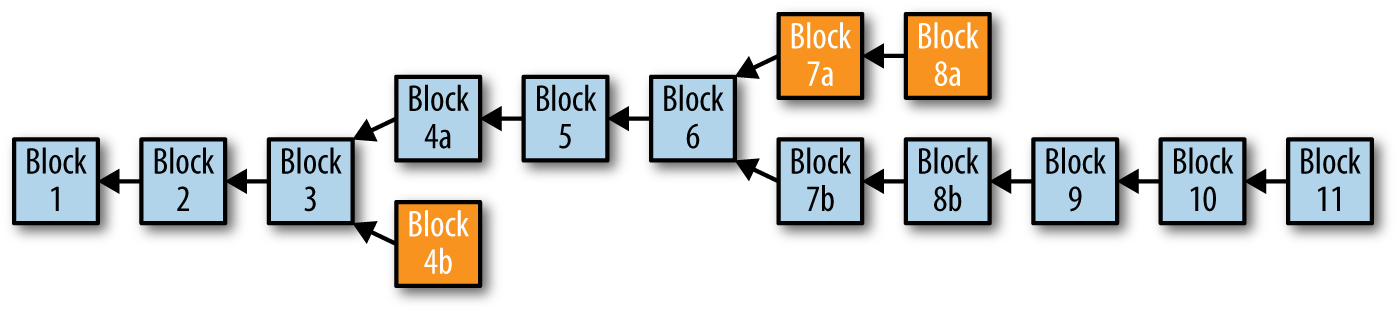
\includegraphics[scale=0.5]{mbc2_1009.png}
    \end{center}
\end{frame}

\begin{frame}
    \frametitle{Block Chain Fork}
    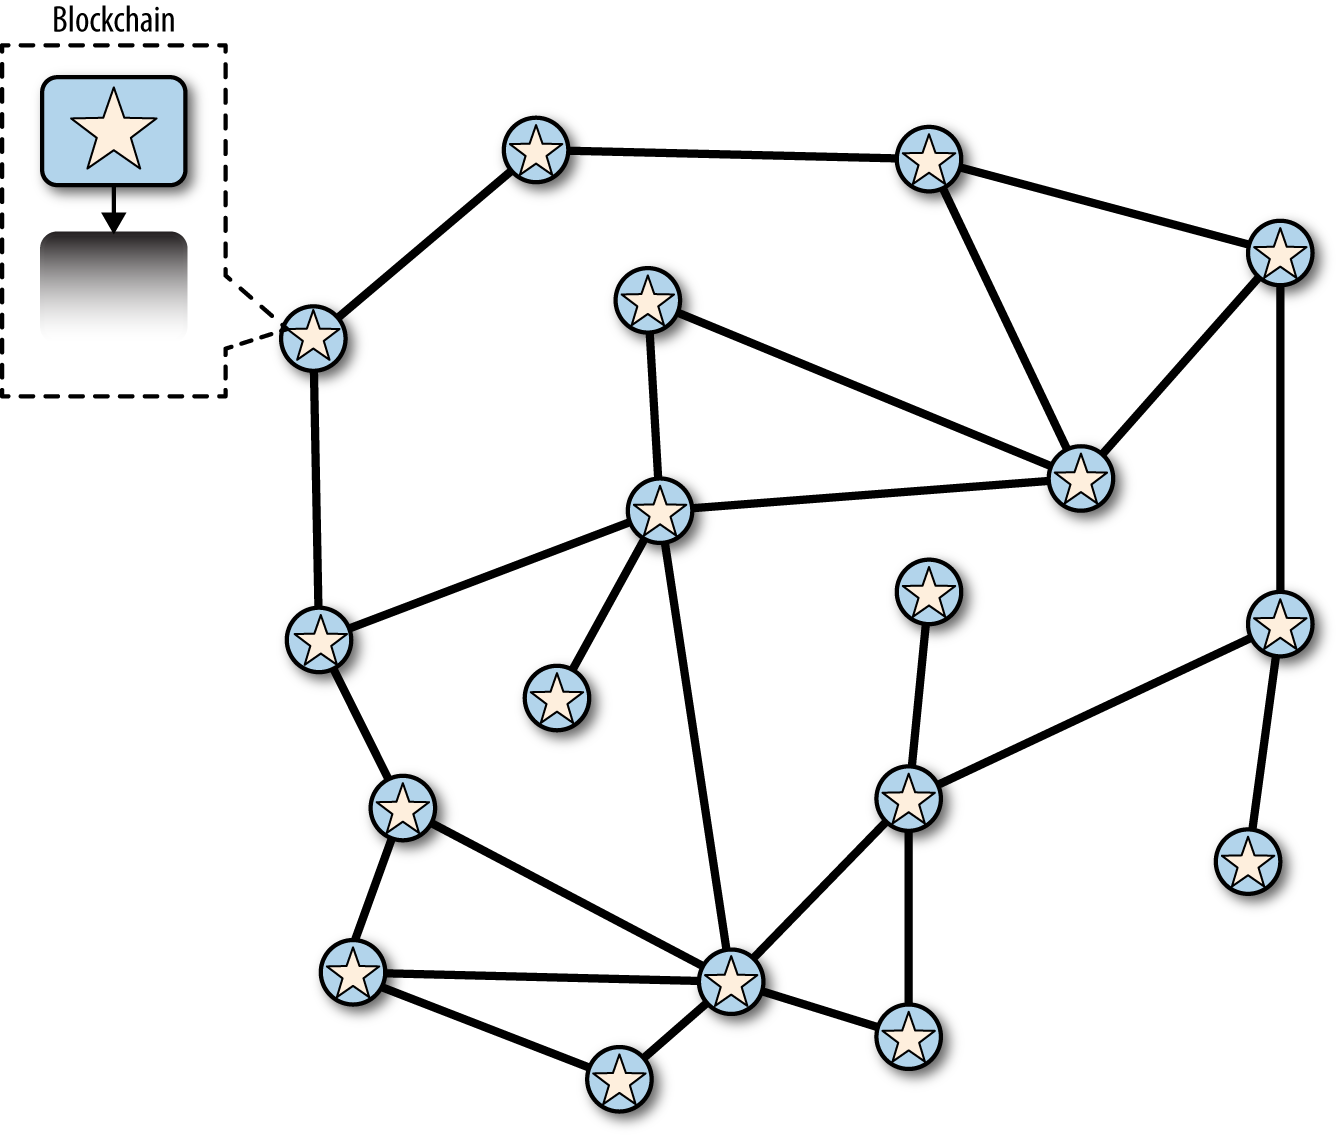
\includegraphics[scale=0.7]{mbc2_1002.png}
\end{frame}

\begin{frame}
    \frametitle{Block Chain Fork}
    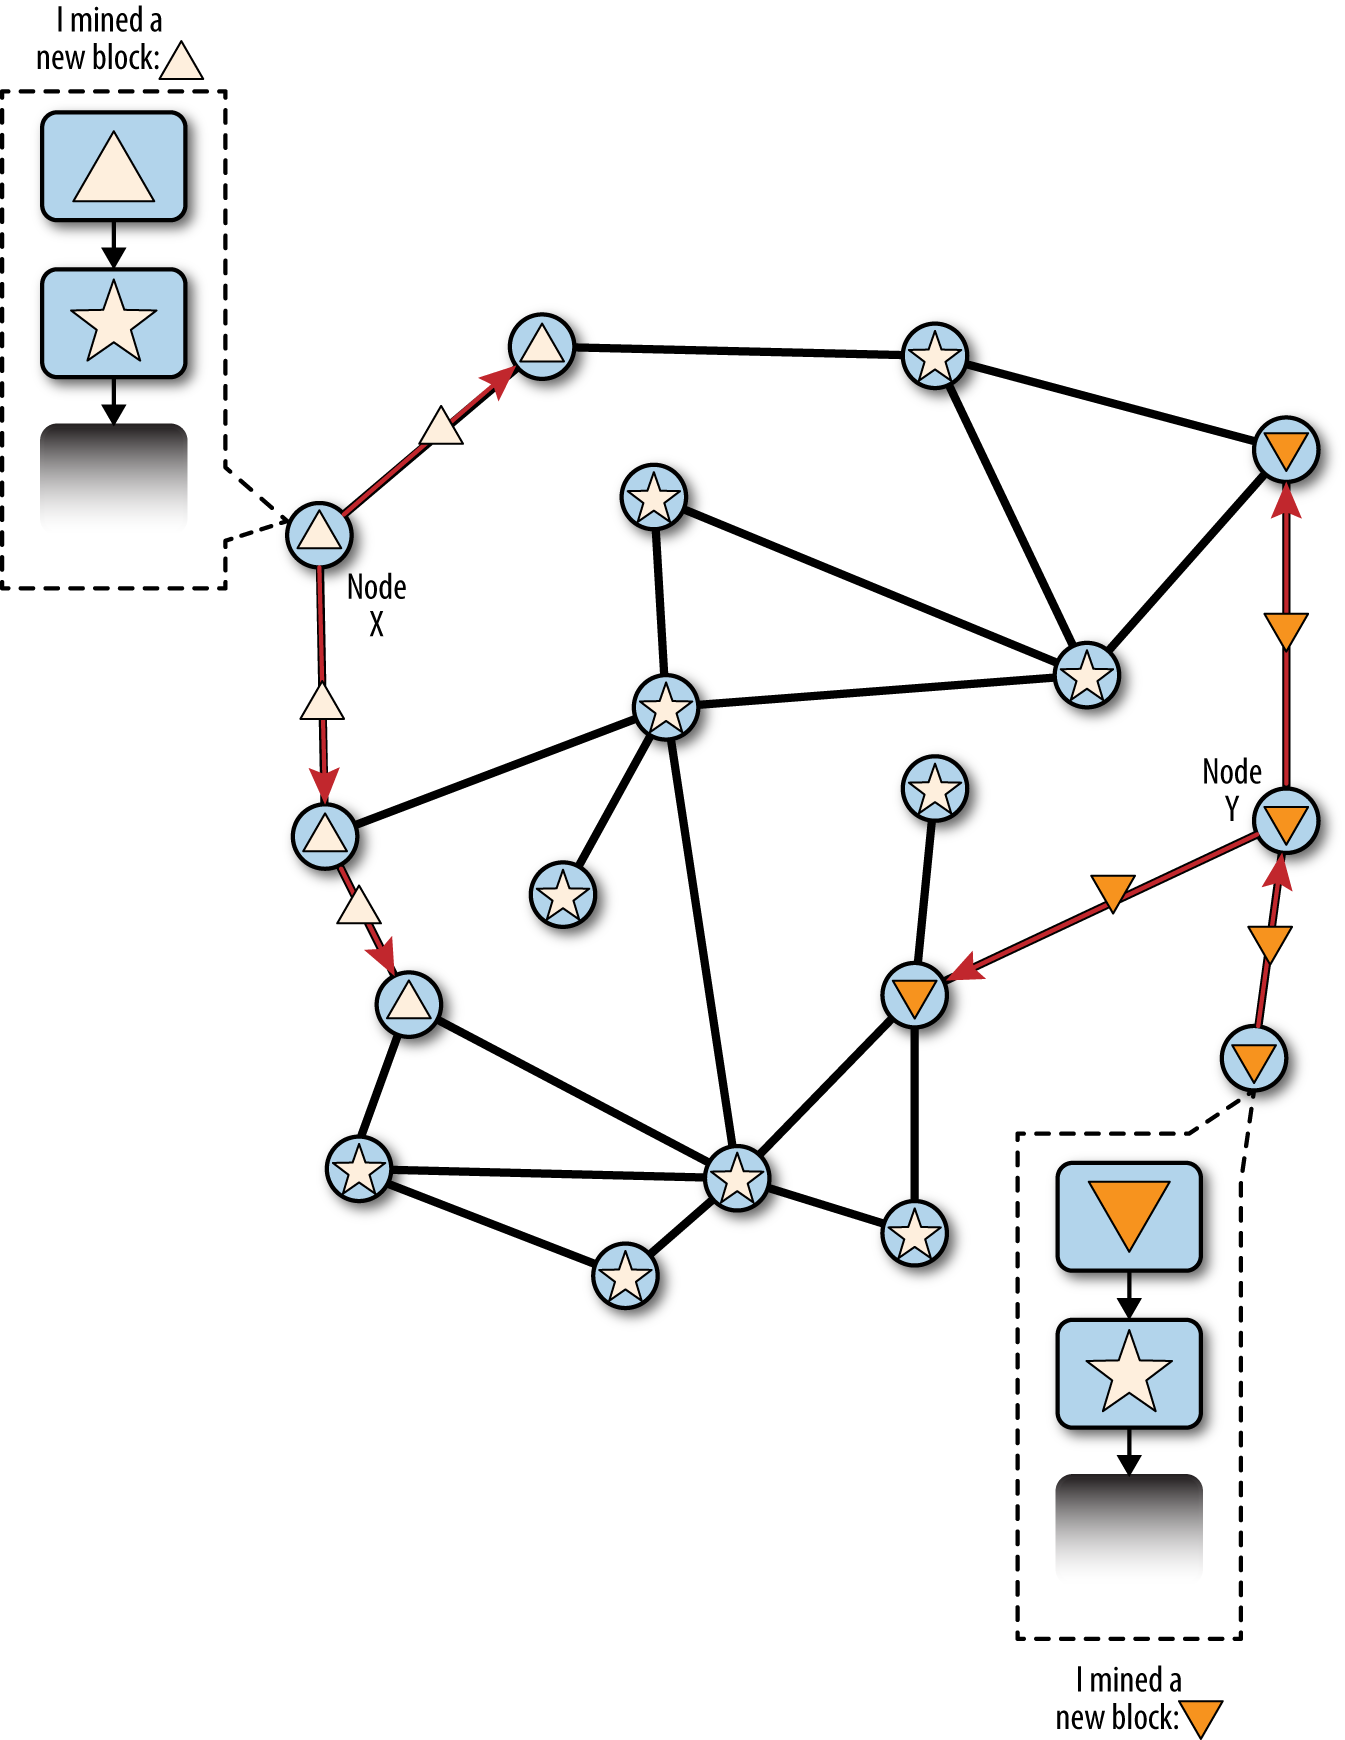
\includegraphics[scale=0.5]{mbc2_1003.png}
\end{frame}

\begin{frame}
    \frametitle{Block Chain Fork}
    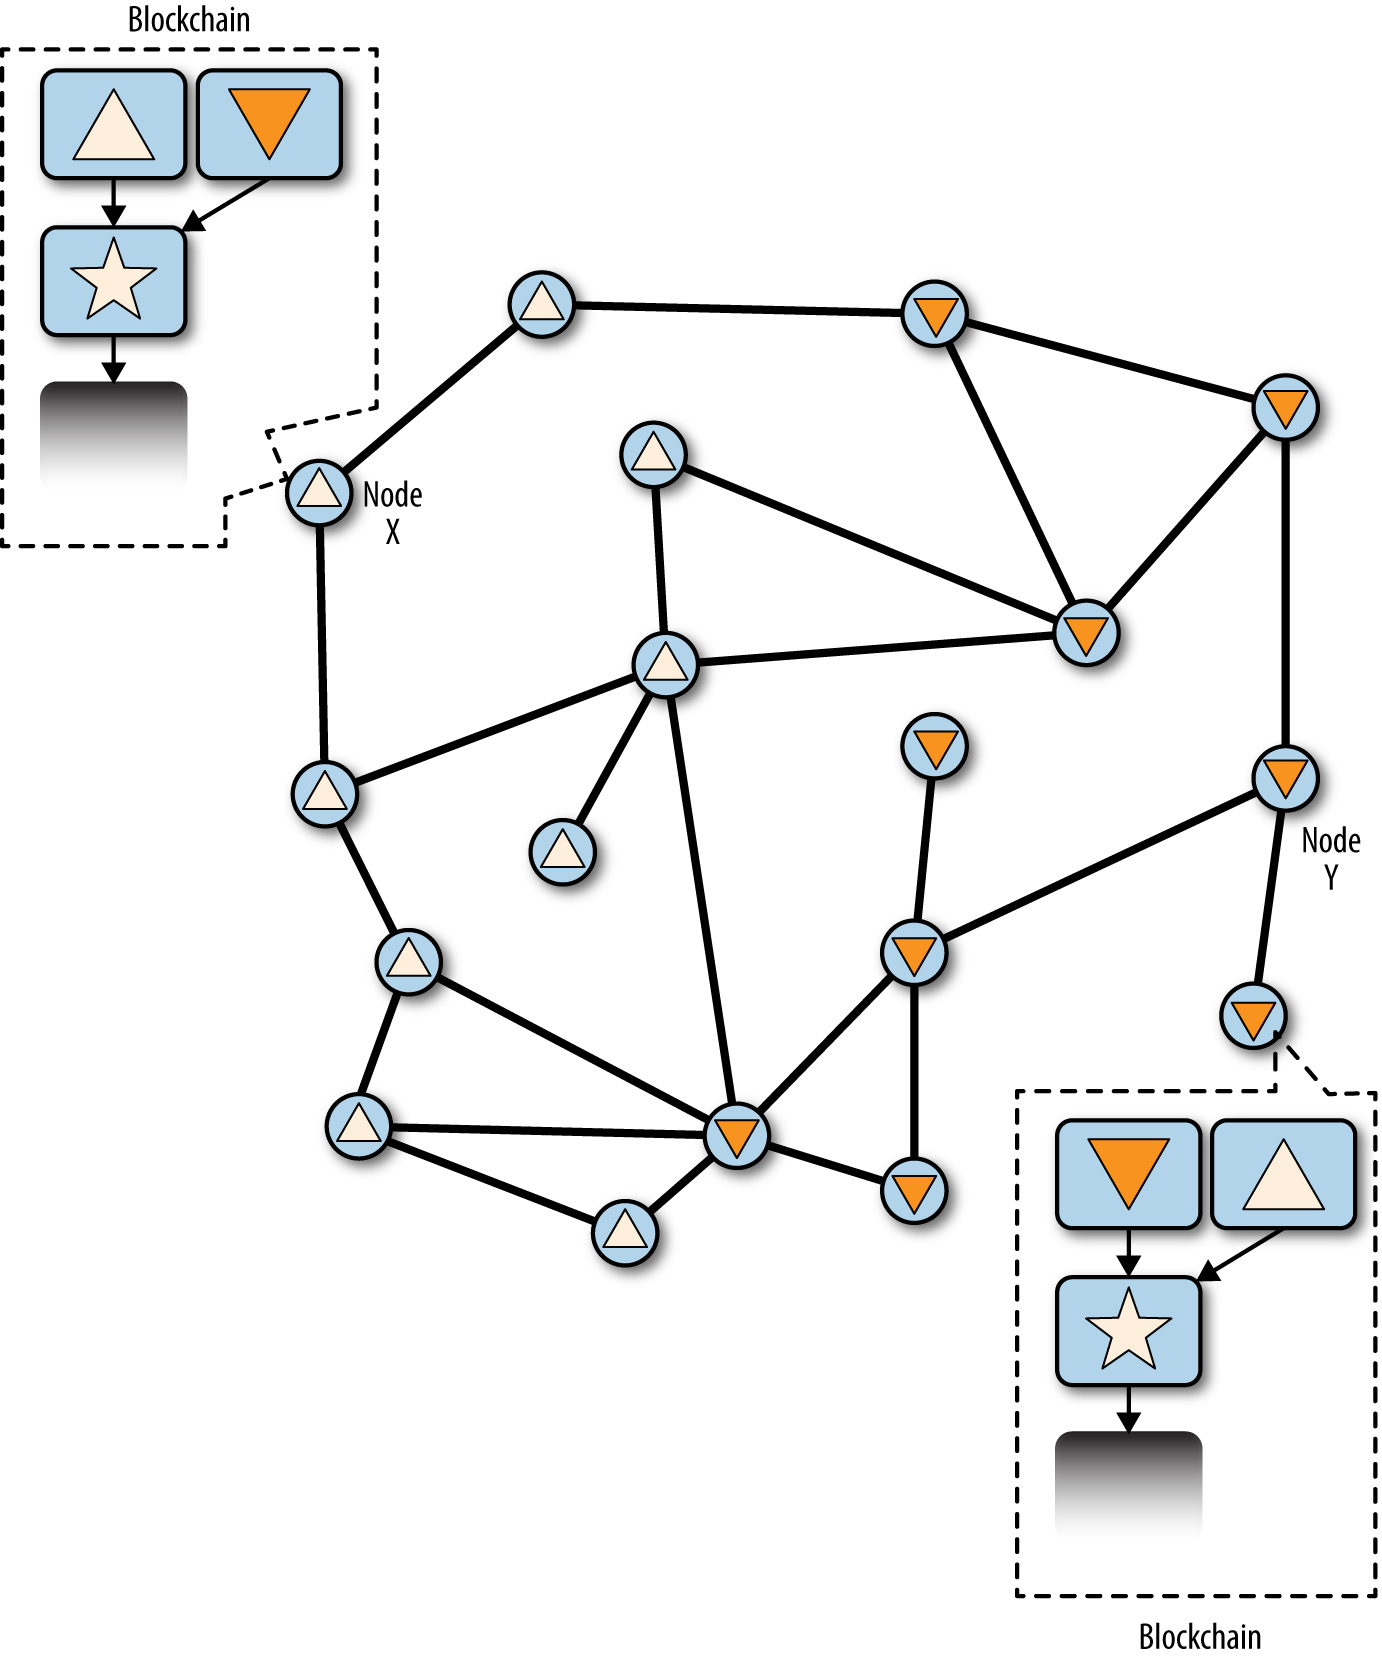
\includegraphics[scale=0.5]{mbc2_1004.png}
\end{frame}

\begin{frame}
    \frametitle{Block Chain Fork}
    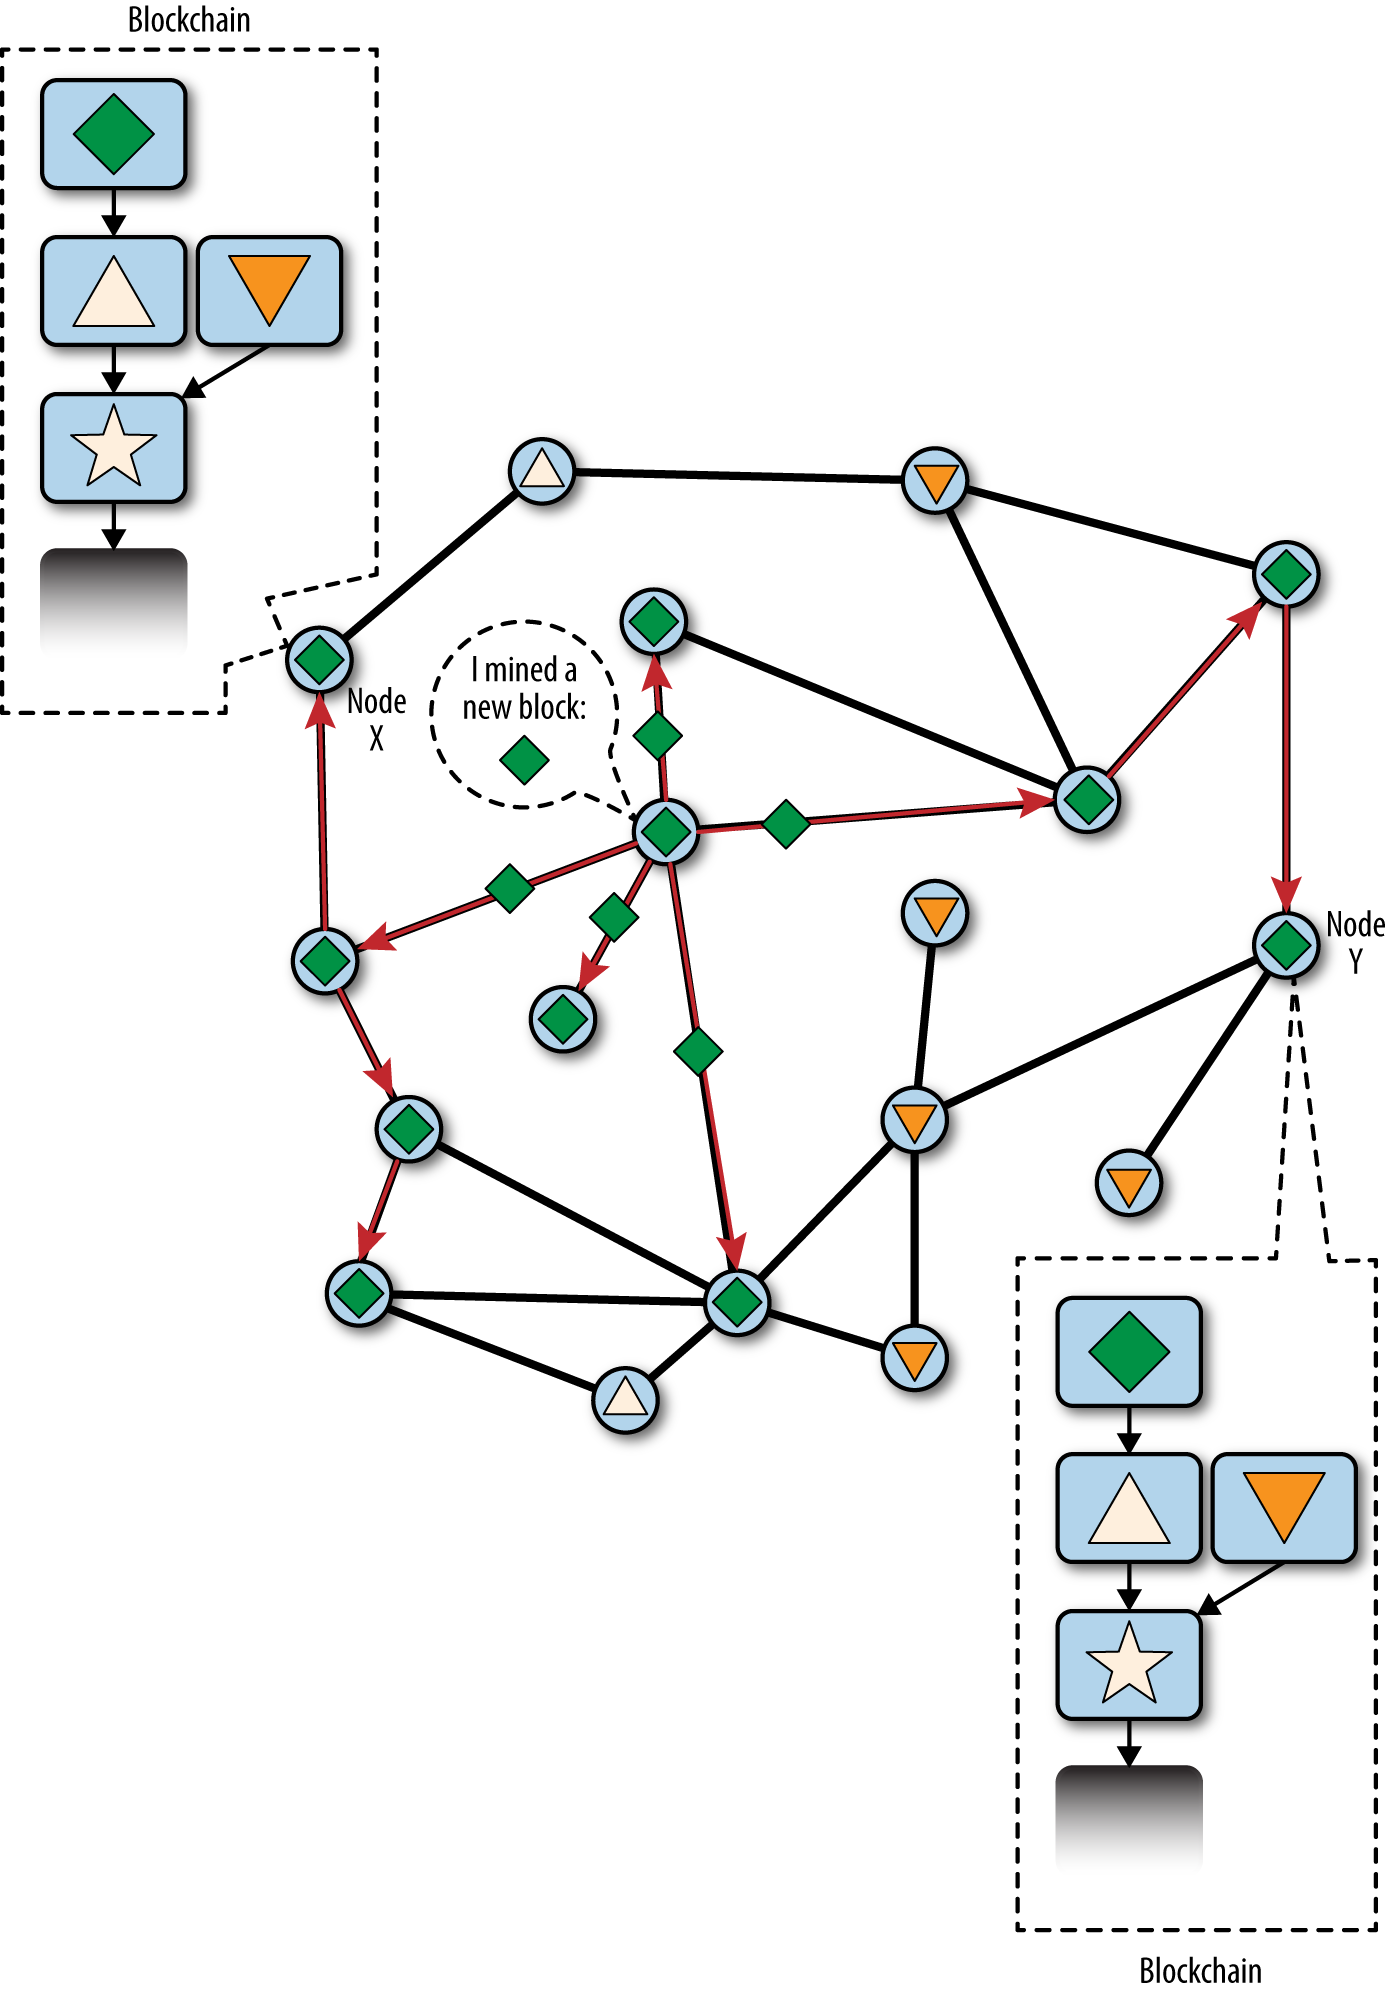
\includegraphics[scale=0.5]{mbc2_1005.png}
\end{frame}

\begin{frame}
    \frametitle{Block Chain Fork}
    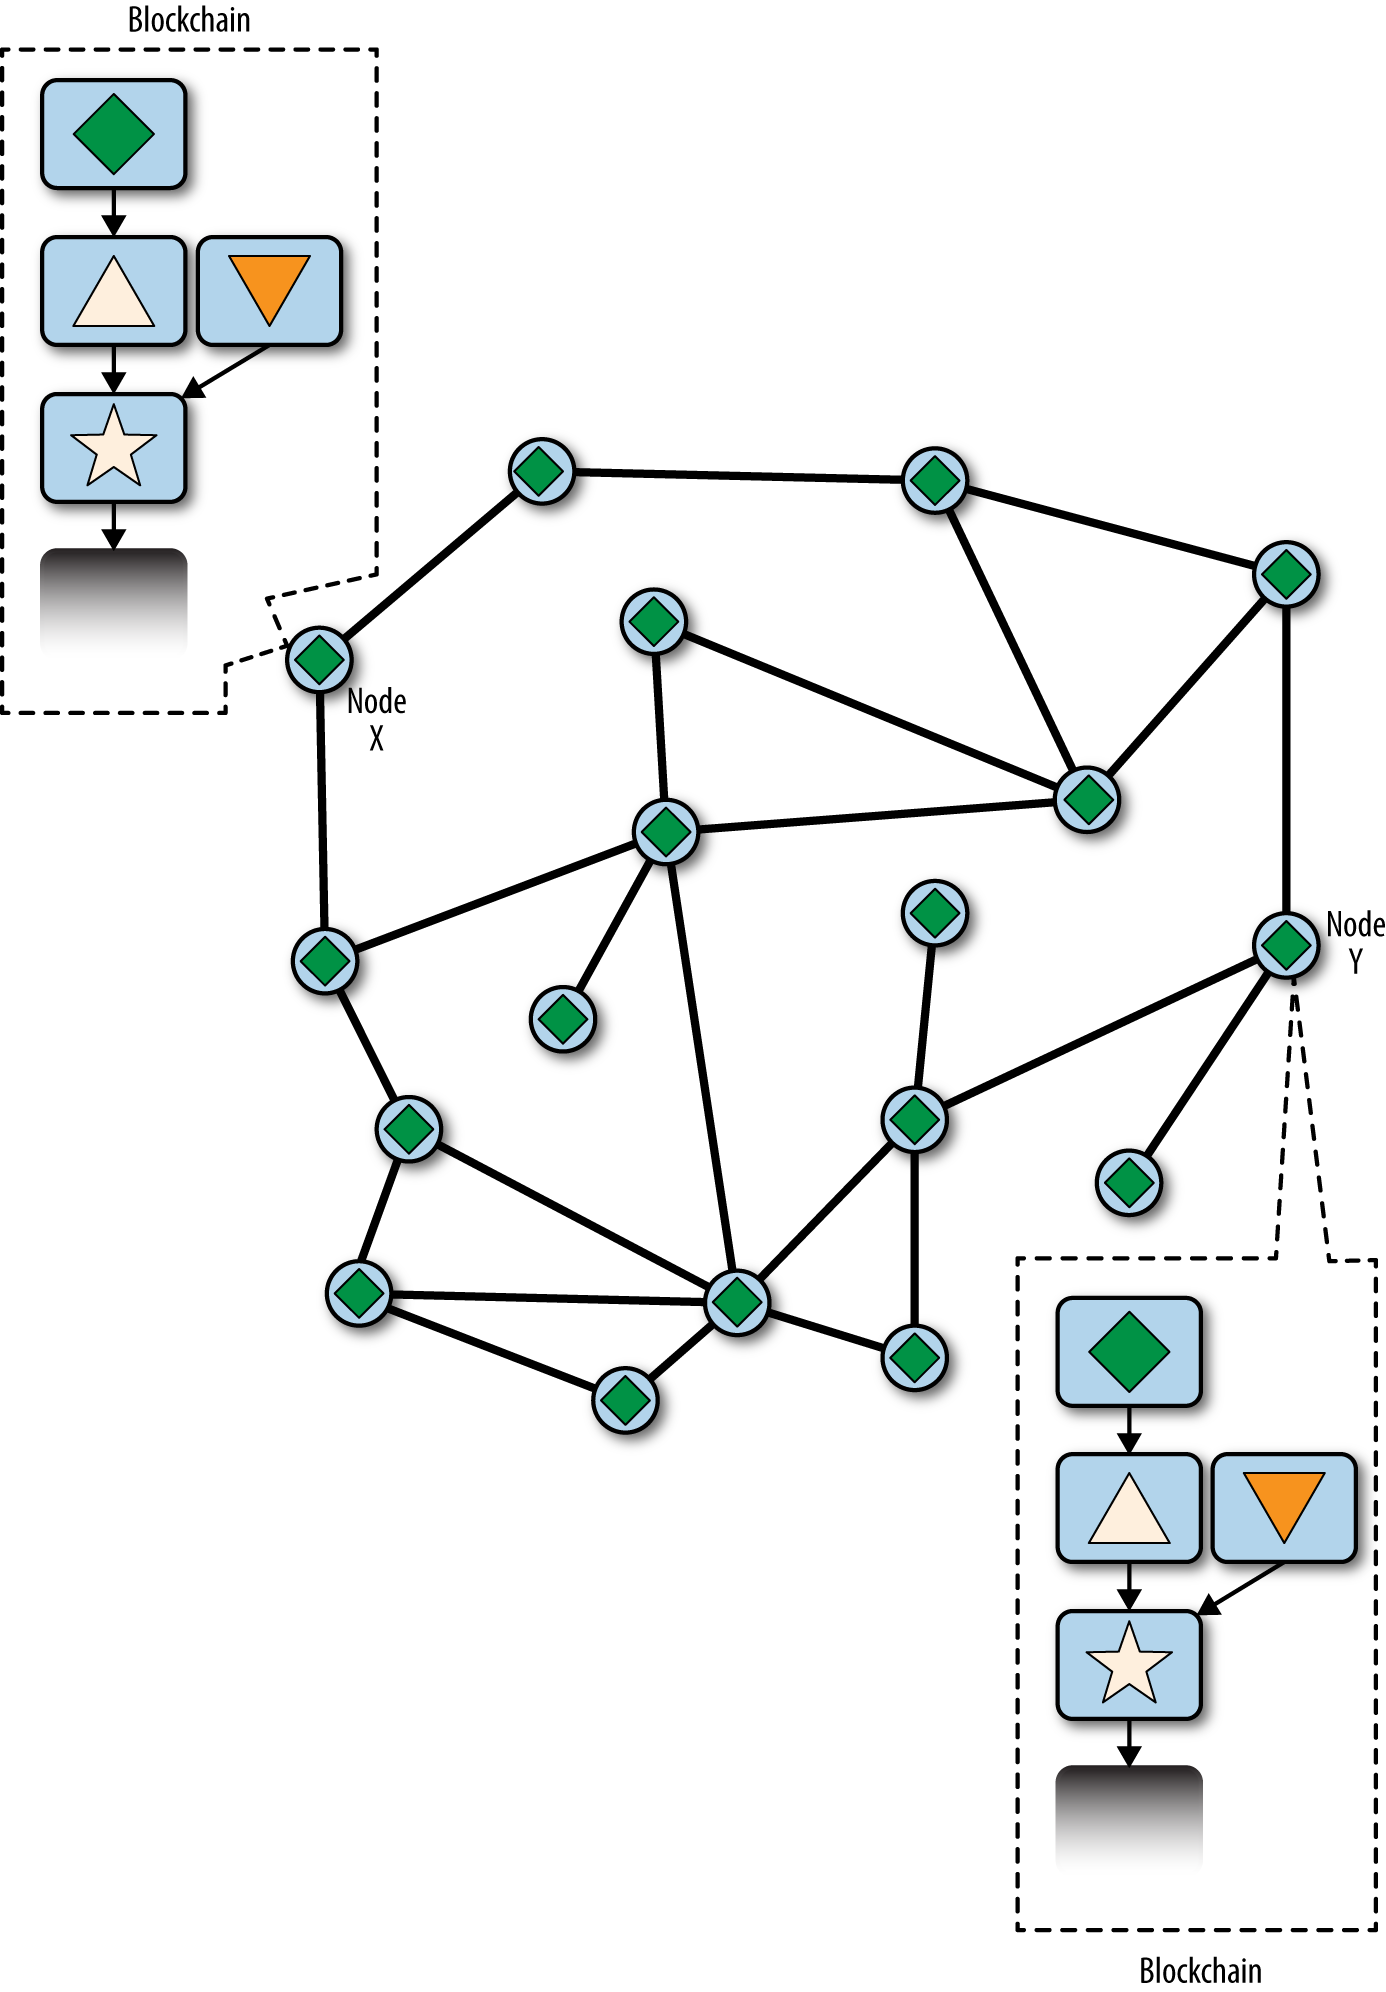
\includegraphics[scale=0.5]{mbc2_1006.png}
\end{frame}

\begin{frame}
    \frametitle{Double Spending Attack}
    Any attacker is competing against the whole network.
    \begin{center}
        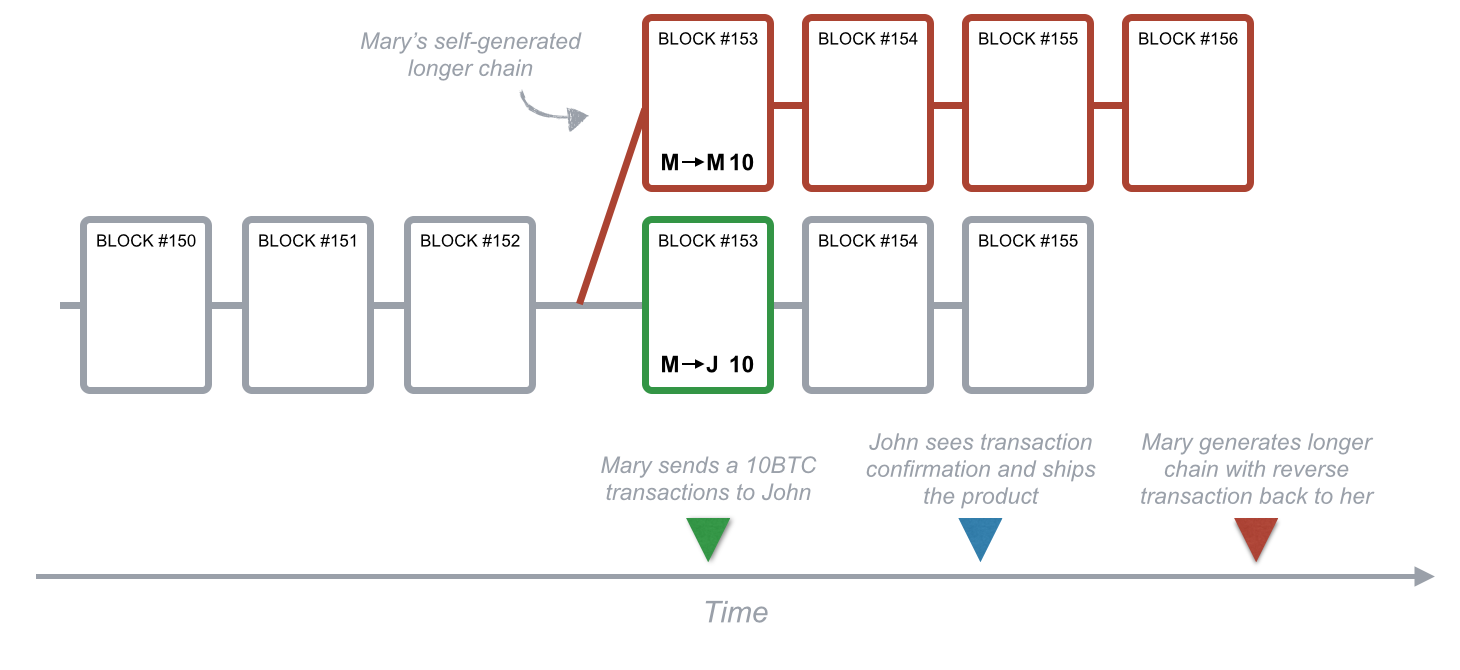
\includegraphics[scale=0.16]{double-spending.png}
    \end{center}
    \begin{itemize}
        \item Each block contains a reference to the previous block.
        \item 51\% computing power of the whole network have a 50\% chance to solve a block before some other node does.
        \item Create 2, 3 or more blocks in a row is even harder.
    \end{itemize}
\end{frame}

\begin{frame}
    \frametitle{Blockchain Transactions Security}
    Transactions get more and more secure with time.
    \begin{itemize}
        \item A block is add to the chain every 10 minutes on average.
        \item Waiting for 6 block(1 hour) gives a quite high probability that the transaction has been processed and is \alert{non reversible}.
    \end{itemize}
    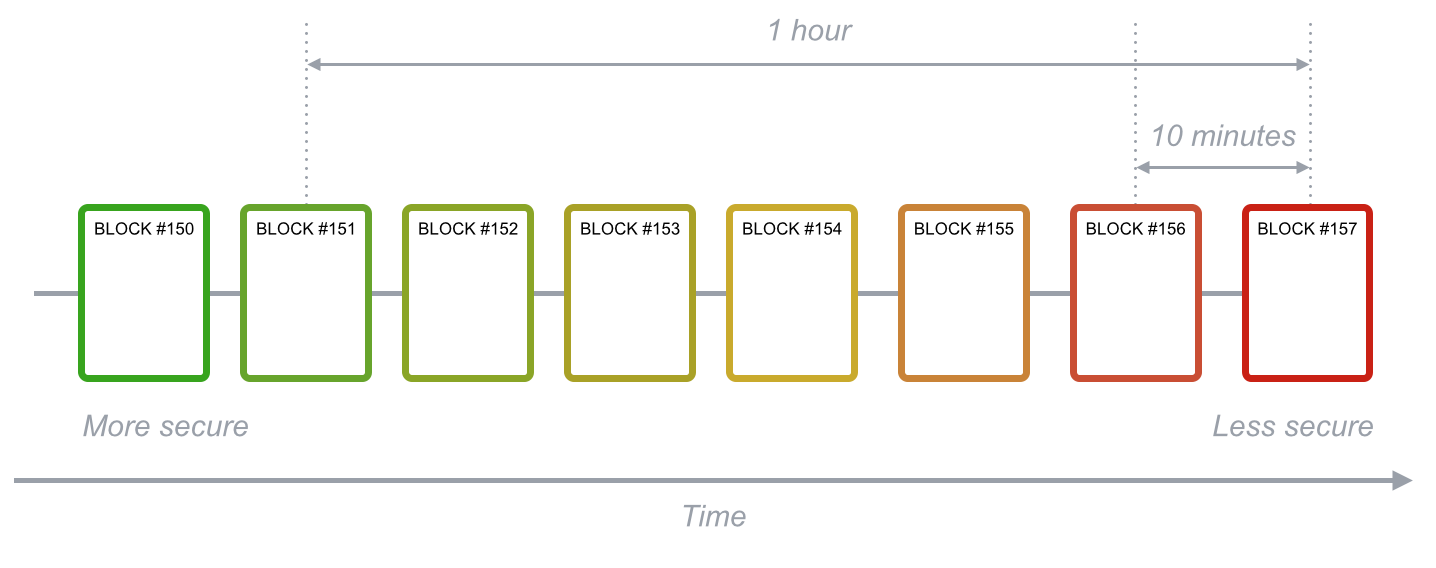
\includegraphics[scale=0.2]{bitcoin-security.png}
\end{frame}

\begin{frame}
    \frametitle{Two Generals' Problem}
    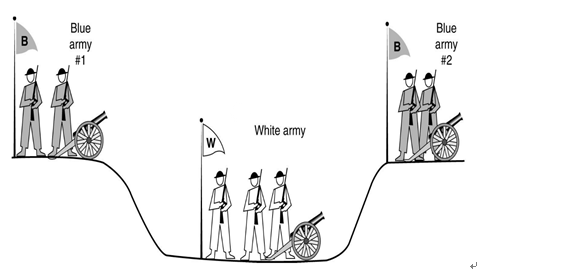
\includegraphics[scale=0.5]{two-generals-problem.png}
    \begin{itemize}
        \item \alert{Two generals} need to coordinate an attack.
            \begin{itemize}
                \item Must \alert{agree} on time to attack.
                \item They will win only if they attack \alert{simultaneously}.
                \item Communicate through \alert{messengers}.
                \item Messengers may be \alert{killed} on their way.
            \end{itemize}
    \end{itemize}
\end{frame}

\begin{frame}
    \frametitle{Two Generals' Problem}
    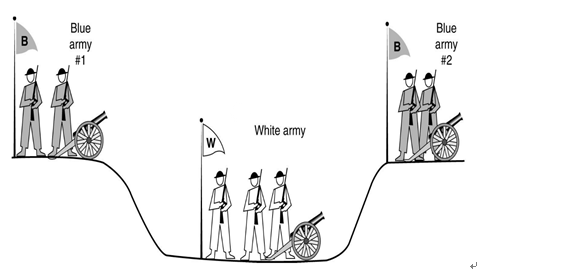
\includegraphics[scale=0.5]{two-generals-problem.png}
    \begin{itemize}
        \item Let's try to solve it for general g1 and g2.
        \item g1 sends \alert{time of attack} to g2.
            \begin{itemize}
                \item \alert{Problem}: how to ensure g2 received message?
                \item \alert{Solution}: let g2 ack receipt of message.
                \item \alert{Problem}: how to ensure g1 received ack?
                \item \alert{Solution}: let g1 ack the receipt of the ack.
                \item \ldots
            \end{itemize}
        \item This problem is \alert{impossible} to solve!
    \end{itemize}
\end{frame}

\begin{frame}
    \frametitle{Engineering approaches: TCP handshake}
    A progmatic approach to dealing with the Two Generals's Problem
    \begin{itemize}
        \item Accept the \alert{uncertainty} of the Communication channel.
        \item Not attempt to eliminate it, but mitigate it to an acceptable degree.
        \item Classic Example is TCP handshake protocol.
    \end{itemize}
    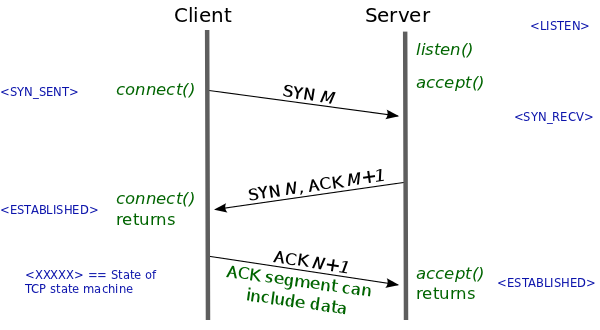
\includegraphics[scale=0.4]{tcp-handshake.png}
\end{frame}


\section{Conclusion}
\section{Conclusions}
\subsection{Conclusions}

\begin{frame}

\end{frame}



%\begin{frame}
    \frametitle{Q \& A}
    \begin{block}{Question}
I don't understand why the blockchain is so important. Isn't the
requirement for the owner's signature on each transaction enough to
prevent bitcoins from being stolen?
    \end{block}
\end{frame}

\begin{frame}
    \frametitle{Q \& A}
    \begin{block}{Question}
I don't understand why the blockchain is so important. Isn't the
requirement for the owner's signature on each transaction enough to
prevent bitcoins from being stolen?
    \end{block}

    \begin{block}{Answer}
The signature is not enough, because it doesn't prevent the owner
from spending money twice: signing two transactions that transfer the
same bitcoin to different recipients. The blockchain acts as a
publishing system to try to ensure that once a bitcoin has been spent
once, lots of participants will know, and will be able to reject a
second spend.
    \end{block}
\end{frame}

\begin{frame}
    \frametitle{Q \& A}
    \begin{block}{Question}
Why does Bitcoin need to define a new currency? Wouldn't it be more
convenient to use an existing currency like dollars?
    \end{block}
\end{frame}

\begin{frame}
    \frametitle{Q \& A}
    \begin{block}{Question}
Why does Bitcoin need to define a new currency? Wouldn't it be more
convenient to use an existing currency like dollars?
    \end{block}

    \begin{block}{Answer}
The new currency (Bitcoins) allows the system to reward miners with
freshly created money; this would be harder with dollars because it's
illegal for ordinary people to create fresh dollars. And using dollars
would require a separate settlement system: if I used the blockchain
to record a payment to someone, I still need to send the recipient
dollars via a bank transfer or physical cash.
    \end{block}
\end{frame}

\begin{frame}
    \frametitle{Q \& A}
    \begin{block}{Question}
Why is the purpose of proof-of-work?
    \end{block}
\end{frame}

\begin{frame}
    \frametitle{Q \& A}
    \begin{block}{Question}
Why is the purpose of proof-of-work?
    \end{block}

    \begin{block}{Answer}
It makes it hard for an attacker to convince the system to switch
to a blockchain fork in which a coin is spent in a different way than
in the main fork. You can view proof-of-work as making a random choice
over the participating CPUs of who gets to choose which fork to
extend. If the attacker controls only a few CPUs, the attacker won't
be able to work hard enough to extend a new malicious fork fast enough
to overtake the main blockchain.
    \end{block}
\end{frame}

\begin{frame}
    \frametitle{Q \& A}
    \begin{block}{Question}
Could a Bitcoin-like system use something less wasteful than
proof-of-work?
    \end{block}
\end{frame}

\begin{frame}
    \frametitle{Q \& A}
    \begin{block}{Question}
Could a Bitcoin-like system use something less wasteful than
proof-of-work?
    \end{block}

    \begin{block}{Answer}
Proof-of-work is hard to fake or simulate, a nice property in a
totally open system like Bitcoin where you cannot trust anyone to
follow rules. There are some alternate schemes; search the web for
proof-of-stake, for example. In a smallish closed system, in which the
participants are known though not entirely trusted, Byzantine
agreement protocols could be used, as in Hyperledger.
    \end{block}
\end{frame}

\begin{frame}
    \frametitle{Q \& A}
    \begin{block}{Question}
Can Alice spend the same coin twice by sending "pay Bob" and "pay
Charlie" to different subsets of miners?
    \end{block}
\end{frame}

\begin{frame}
    \frametitle{Q \& A}
    \begin{block}{Question}
Can Alice spend the same coin twice by sending "pay Bob" and "pay
Charlie" to different subsets of miners?
    \end{block}

    \begin{block}{Answer}
The most likely scenario is that one subset of miners finds the
nonce for a new block first. Let's assume the first block to be found
is B50 and it contains "pay Bob". This block will be flooded to all
miners, so the miners working on "pay Charlie" will switch to mining a
successor block to B50. These miners validate transactions they place
in blocks, so they will notice that the "pay Charlie" coin was spent in
B50, and they will ignore the "pay Charlie" transaction. Thus, in this
scenario, double-spend won't work.

There's a small chance that two miners find blocks at the same time,
perhaps B50' containing "pay Bob" and B50'' containing "pay Charlie". At
this point there's a fork in the block chain. These two blocks will be
flooded to all the nodes. Each node will start mining a successor to one
of them (the first it hears). Again the most likely outcome is that a
single miner will finish significantly before any other miner, and flood
the successor, and most peers will switch that winning fork. The chance
of repeatedly having two miners simultaneously find blocks gets very
small as the forks get longer. So eventually all the peers will switch
to the same fork, and in fork there will be only one spend of the coin.

The possibility of accidentally having a short-lived fork is the reason
that careful clients will wait until there are a few successor blocks
before believing a transaction.
    \end{block}
\end{frame}

\begin{frame}
Q: It takes an average of 10 minutes for a Bitcoin block to be
validated. Does this mean that the parties involved aren't sure if the
transaction really happened until 10 minutes later?
 
A: The 10 minutes is awkward. But it's not always a problem. For
example, suppose you buy a toaster oven with Bitcoin from a web site.
The web site can check that the transaction is known by a few servers,
though not yet in a block, and show you a "purchase completed" page.
Before shipping it to you, they should check that the transaction is
in a block. For low-value in-person transactions, such as buying a cup
of coffee, it's probably enough for the seller to ask a few peers to
check that the bitcoins haven't already been spent (i.e. it's
reasonably safe to not bother waiting for the transaction to appear in
the blockchain at all).
\end{frame}

\begin{frame}
Q: What can be done to speed up transactions on the blockchain?
 
A: I think the constraint here is that 10 minutes needs to be much
larger (i.e. >= 10x) than the time to broadcast a newly found block to
all peers. The point of that is to minimize the chances of two peers
finding new blocks at about the same time, before hearing about the
other peer's block. Two new blocks at the same time is a fork; forks
are bad since they cause disagreement about which transactions are
real, and they waste miners' time. Since blocks can be pretty big (up
to a megabyte), and peers could have slow Internet links, and the
diameter of the peer network might be large, it could easily take a
minute to flood a new block. If one could reduce the flooding time,
then the 10 minutes could also be reduced.
\end{frame}

\begin{frame}
Q: The entire blockchain needs to be downloaded before a node can
participate in the network. Won't that take an impractically long time
as the blockchain grows?

A: It's true that it takes a while for a new node to get all the
transactions. But once a given server has done this work, it can save
the block chain, and doesn't need to fetch it again. It only needs to
know about new blocks, which is not a huge burden. I think most
ordinary users of Bitcoin won't run full Bitcoin nodes; instead they
will one way or another trust some full nodes.
\end{frame}

\begin{frame}
Q: Is it feasible for an attacker to gain a majority of the computing
power among peers?

A: It may be feasible; some people think that big cooperative groups
of miners have been close to a majority at times:
http://www.coindesk.com/51-attacks-real-threat-bitcoin/
\end{frame}




\end{document}



\section{Crypto}
\begin{frame}
    \frametitle{Security in Bitcoin}
    \begin{itemize}
        \item \textbf{Authentication}
            \begin{itemize}
                \item Am I paying the right person?
            \end{itemize}
        \item \textbf{Integrity}
            \begin{itemize}
                \item Is the coin double-spent?
                \item Can an attacker reverse or change transactions?
            \end{itemize}
        \item \textbf{Availability}
            \begin{itemize}
                \item Can I make a transactions anytime I want?
            \end{itemize}
        \item \textbf{Confidentiality}
            \begin{itemize}
                \item Are my transactions private? Anonymous?
            \end{itemize}
    \end{itemize}
\end{frame}

\begin{frame}
    \frametitle{Security in Bitcoin}
    \begin{itemize}
        \item \textbf{Authentication -> \alert{Public Key Crypto: Digital Signatures}}
            \begin{itemize}
                \item Am I paying the right person?
            \end{itemize}
        \item \textbf{Integrity -> \alert{Digital Signatures and Cryptographic Hash}}
            \begin{itemize}
                \item Is the coin double-spent?
                \item Can an attacker reverse or change transactions?
            \end{itemize}
        \item \textbf{Availability -> \alert{Broadcast messages to the P2P network}}
            \begin{itemize}
                \item Can I make a transactions anytime I want?
            \end{itemize}
        \item \textbf{Confidentiality -> \alert{Pesudonymity}}
            \begin{itemize}
                \item Are my transactions private? Anonymous?
            \end{itemize}
    \end{itemize}
\end{frame}

\begin{frame}
    \frametitle{Cryptographic Hash Function}
    \begin{itemize}
        \item \textbf{Computationally efficient}
        \item \textbf{Consistent} \\
            hash(x) always yields same result.
        \item \textbf{Collision Resistant} \\
            Given $hash(W) = Z$, hard to find X such that $hash(X) = Z$
        \item \textbf{One-way} \\
            Given Y, hard to find X s.t. $hash(X) = Y$
    \end{itemize}
    \begin{columns}
        \begin{column}{0.5\textwidth}
            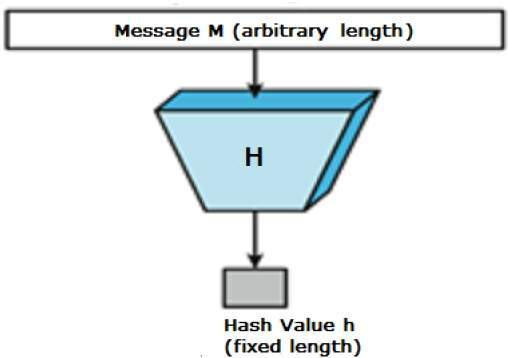
\includegraphics[scale=0.3]{hash_functions.jpg}
        \end{column}
        \begin{column}{0.5\textwidth}
            Common Hash Functions:
            \begin{itemize}
                \item \textbf{MD5}
                \item \textbf{SHA-1}
                \item \textbf{SHA-2}
                    \begin{itemize}
                        \item SHA-256
                        \item SHA-384
                        \item SHA-512
                    \end{itemize}
            \end{itemize}
        \end{column}
    \end{columns}
\end{frame}

\begin{frame}[fragile]
    \frametitle{Hash Function Example}
    \begin{lstlisting}[language=Python]
    SHA224("")
    0x d14a028c2a3a2bc9476102bb288234c415a2b01f828ea62ac5b3e42f
    SHA256("")
    0x e3b0c44298fc1c149afbf4c8996fb92427ae41e4649b934ca495991b7852b855
    \end{lstlisting}

    Even a small change in the message wil result in a mostly different hash.
    \begin{lstlisting}[language=Python]
    SHA224("The quick brown fox jumps over the lazy dog")
    0x 730e109bd7a8a32b1cb9d9a09aa2325d2430587ddbc0c38bad911525
    SHA224("The quick brown fox jumps over the lazy dog.")
    0x 619cba8e8e05826e9b8c519c0a5c68f4fb653e8a3d8aa04bb2c8cd4c
    \end{lstlisting}

    Proof of work first sight:

    Given a basic string \alert{hello world!} + random number \alert{nonce}

    We need the digest have 4 leading 0.
    \begin{lstlisting}[language=Python]
    "Hello, world!0" => 1312af178c253f84028d480a6adc1e25e81caa44c749ec81976192e2ec934c64
    "Hello, world!1" => e9afc424b79e4f6ab42d99c81156d3a17228d6e1eef4139be78e948a9332a7d8
    "Hello, world!2" => ae37343a357a8297591625e7134cbea22f5928be8ca2a32aa475cf05fd4266b7
    ...
    "Hello, world!4248" => 6e110d98b388e77e9c6f042ac6b497cec46660deef75a55ebc7cfdf65cc0b965
    "Hello, world!4249" => c004190b822f1669cac8dc37e761cb73652e7832fb814565702245cf26ebb9e6
    "Hello, world!4250" => 0000c3af42fc31103f1fdc0151fa747ff87349a4714df7cc52ea464e12dcd4e9
    \end{lstlisting}
\end{frame}

\begin{frame}
    \frametitle{Public Key Crypto: Encryption}
    Key pair: Public Key and Private Key
    \begin{columns}
        \begin{column}{0.35\textwidth}
            \begin{center}
                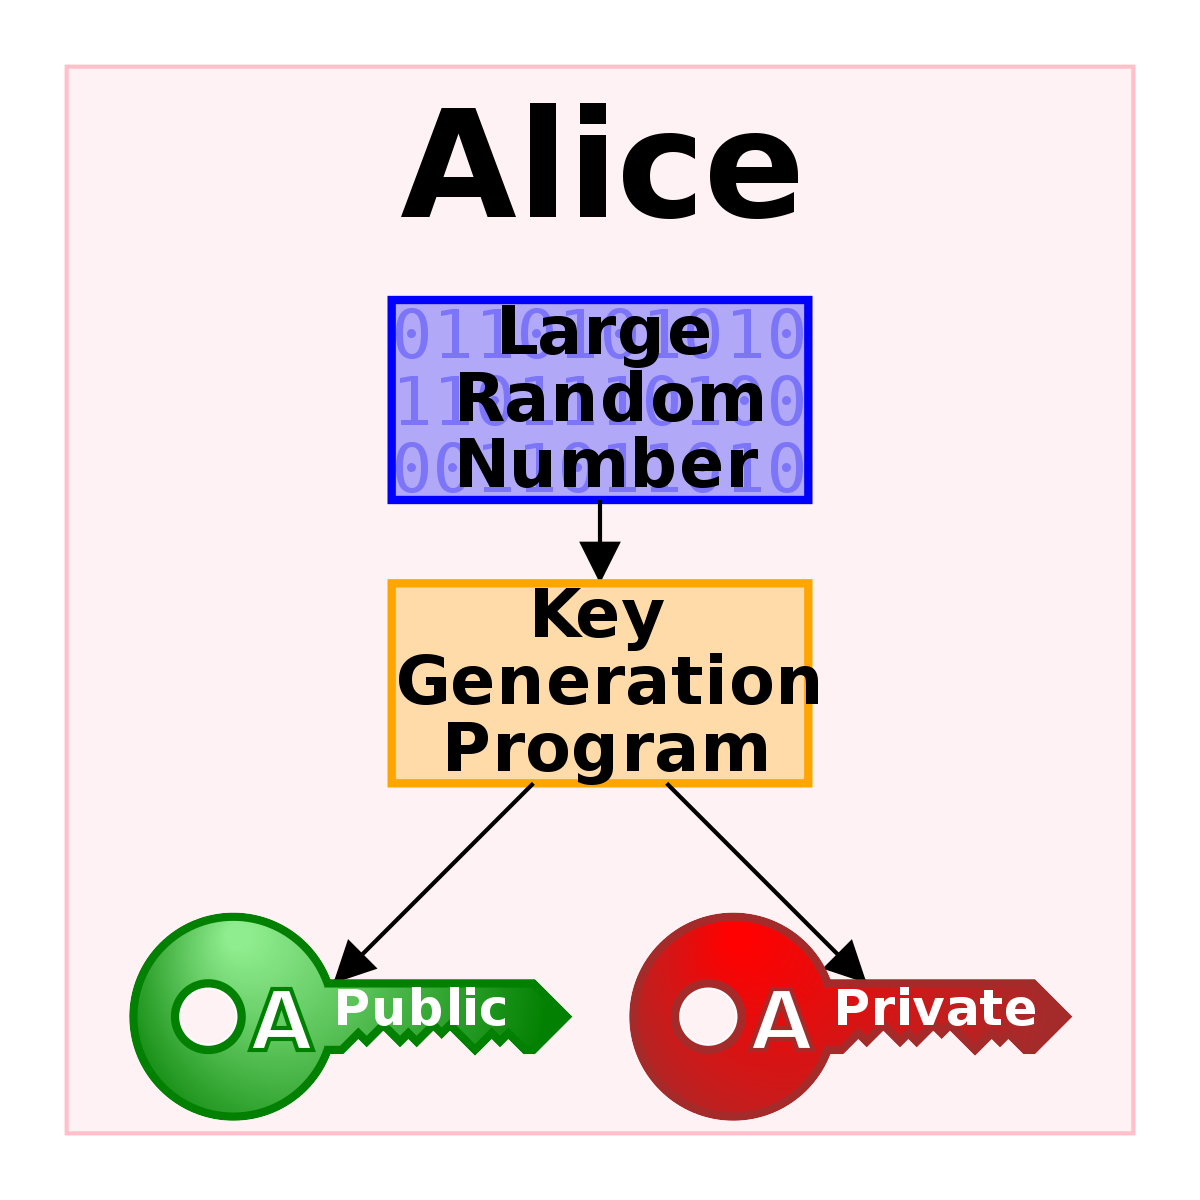
\includegraphics[scale=0.1]{Public-key-crypto.png}
            \end{center}
        \end{column}
        \begin{column}{0.65\textwidth}
            \begin{center}
                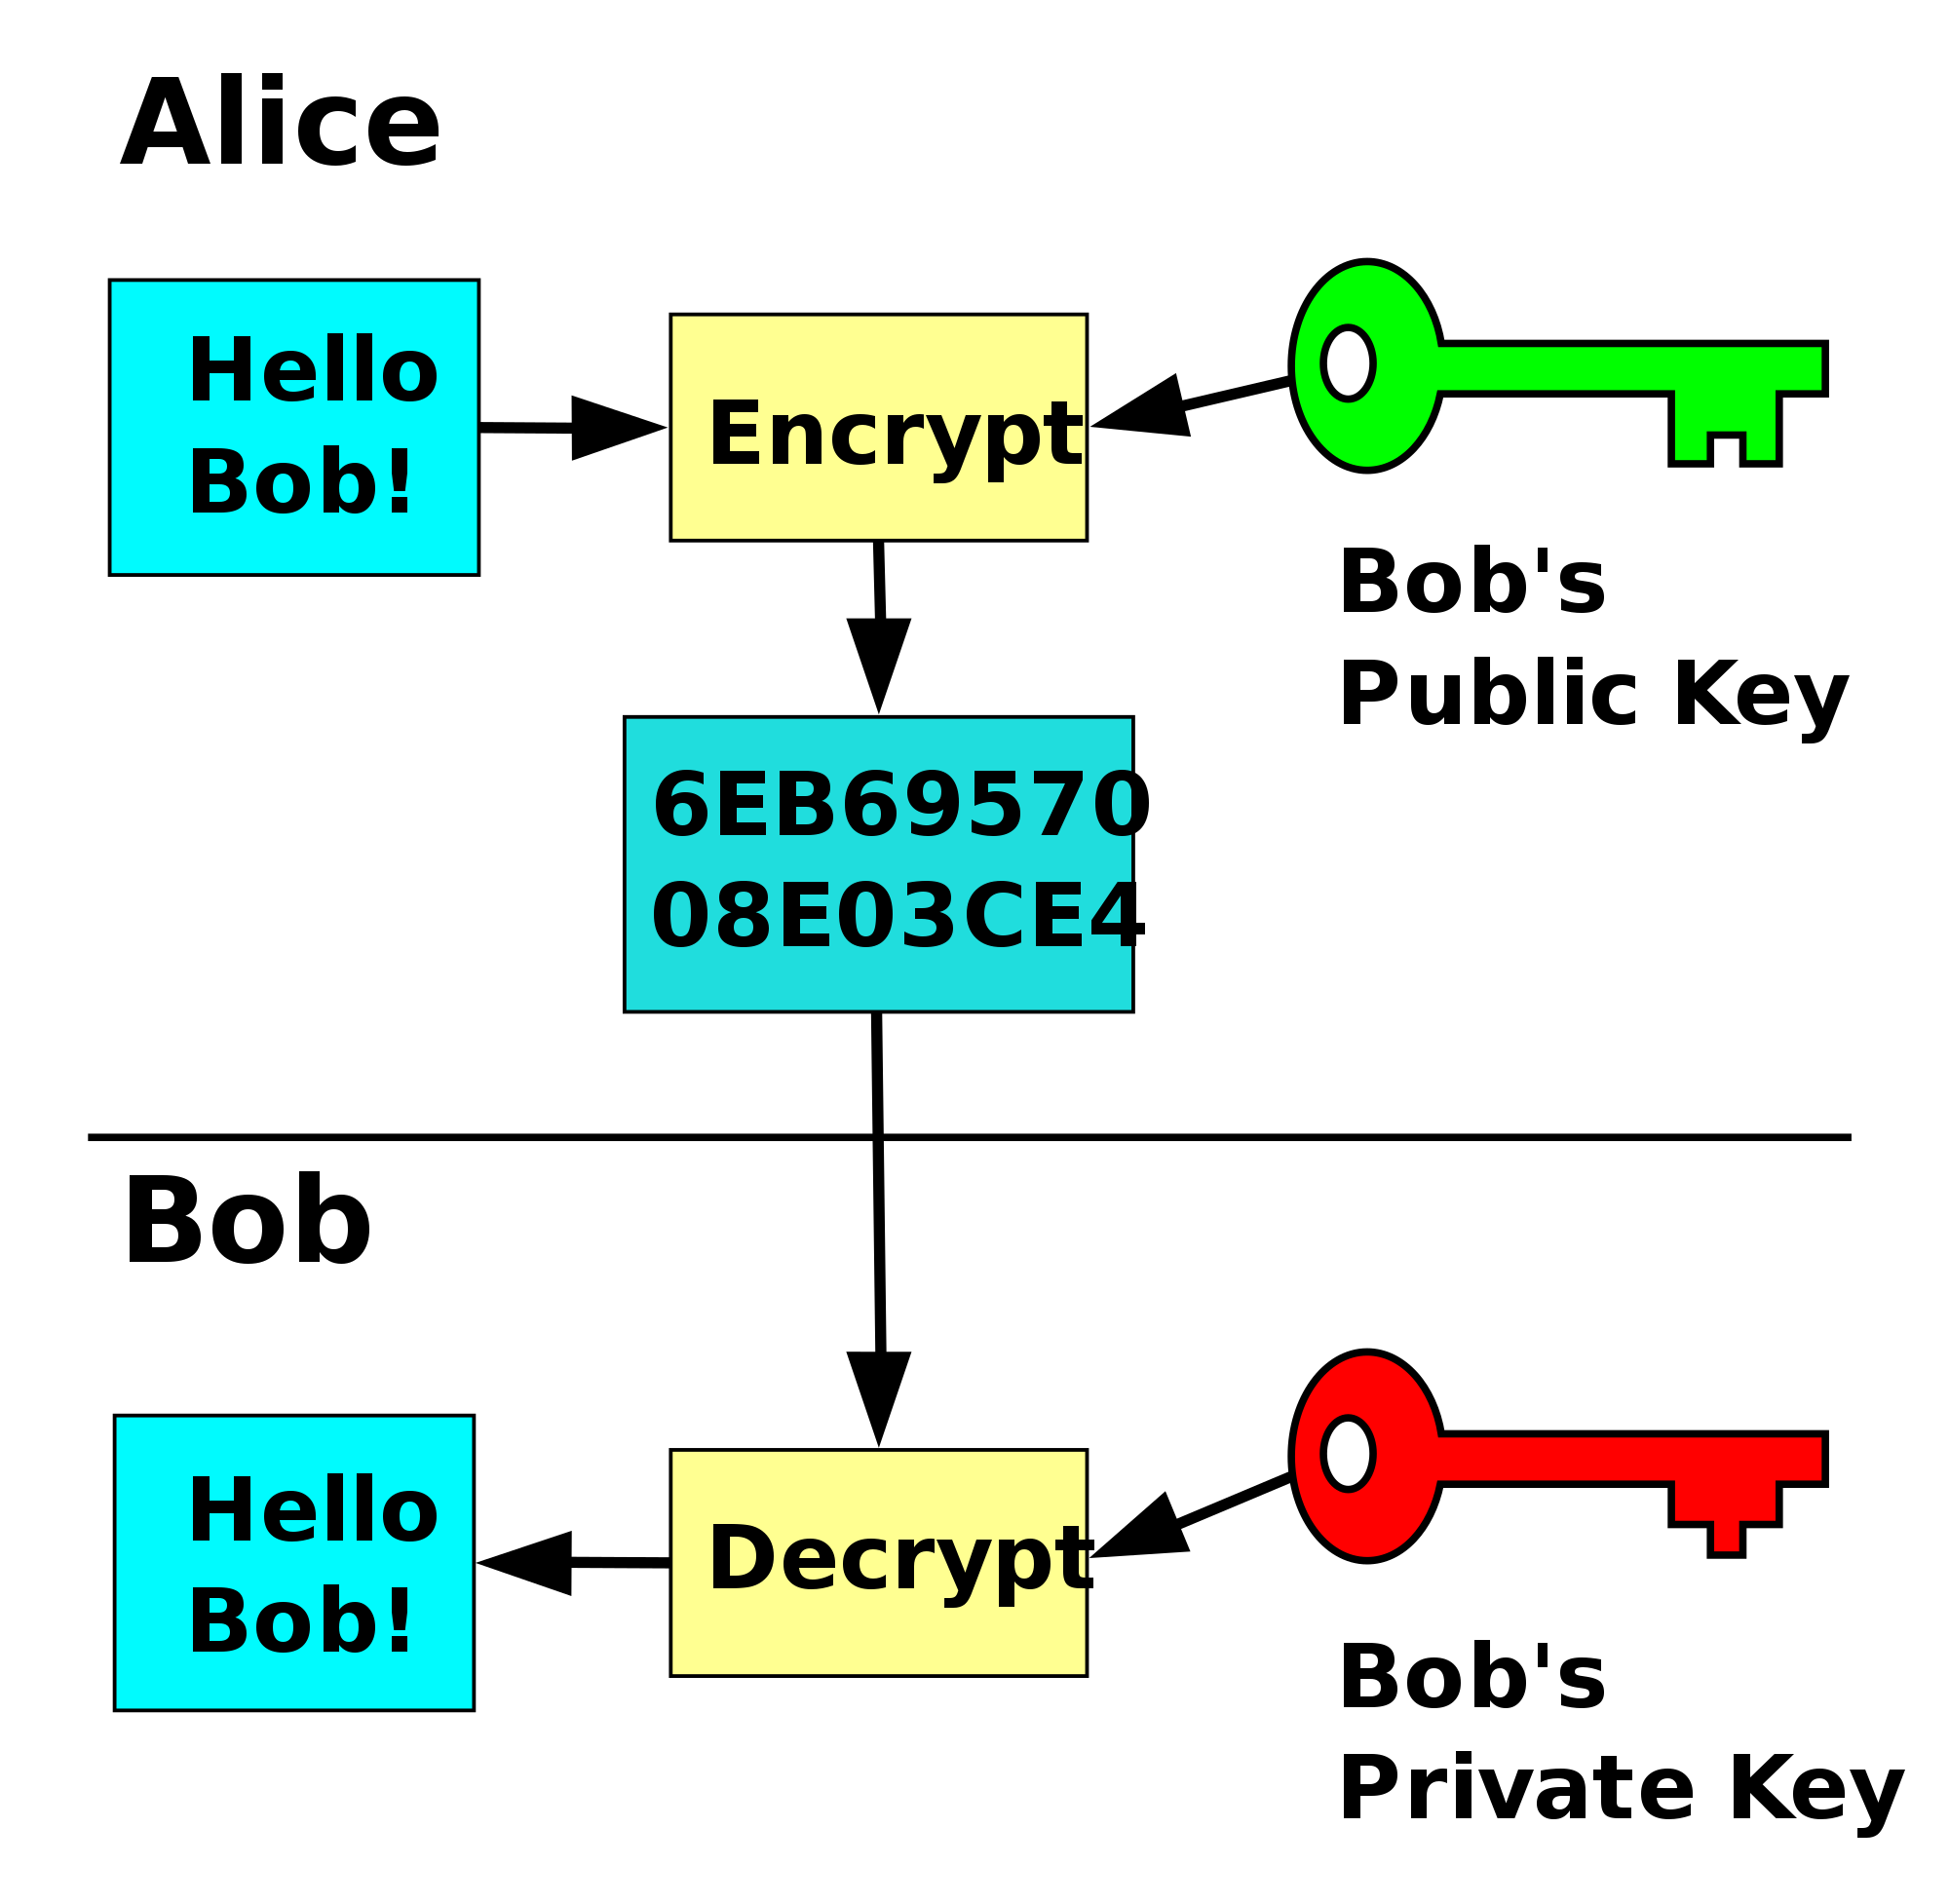
\includegraphics[scale=0.1]{Public_key_shared_secret.png}
            \end{center}
        \end{column}
    \end{columns}
\end{frame}

\begin{frame}
    \frametitle{Public Key Crypto: Digital Signature}
    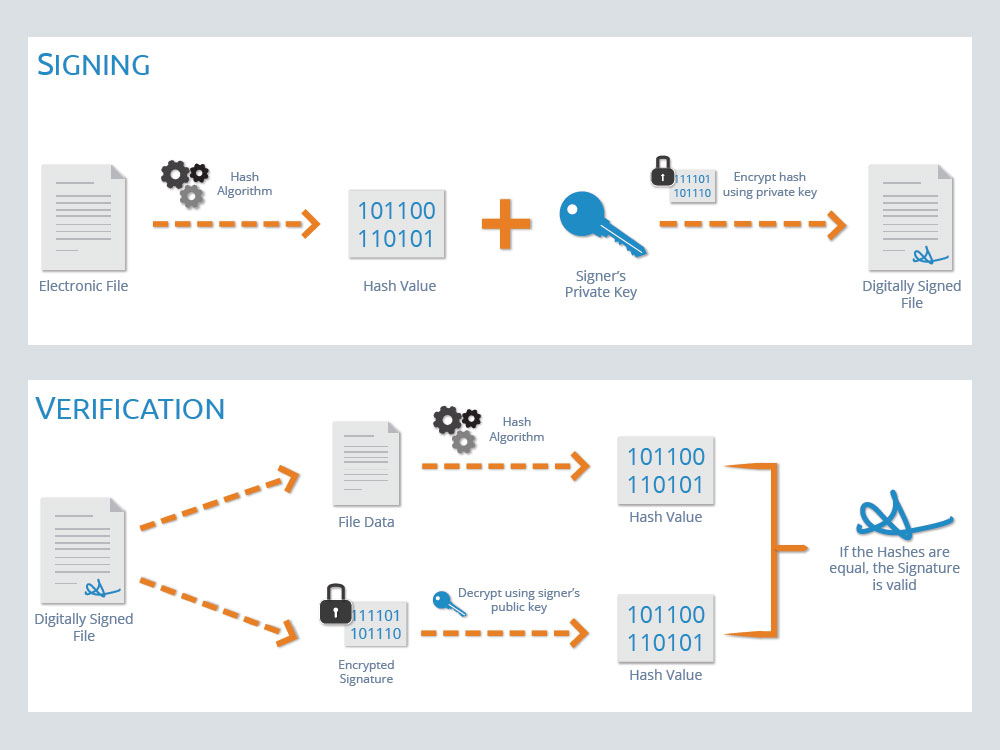
\includegraphics[scale=0.3]{digital-signatures-methodology.jpg}
\end{frame}

\begin{frame}
    \frametitle{Public Key to Bitcoin Address}
    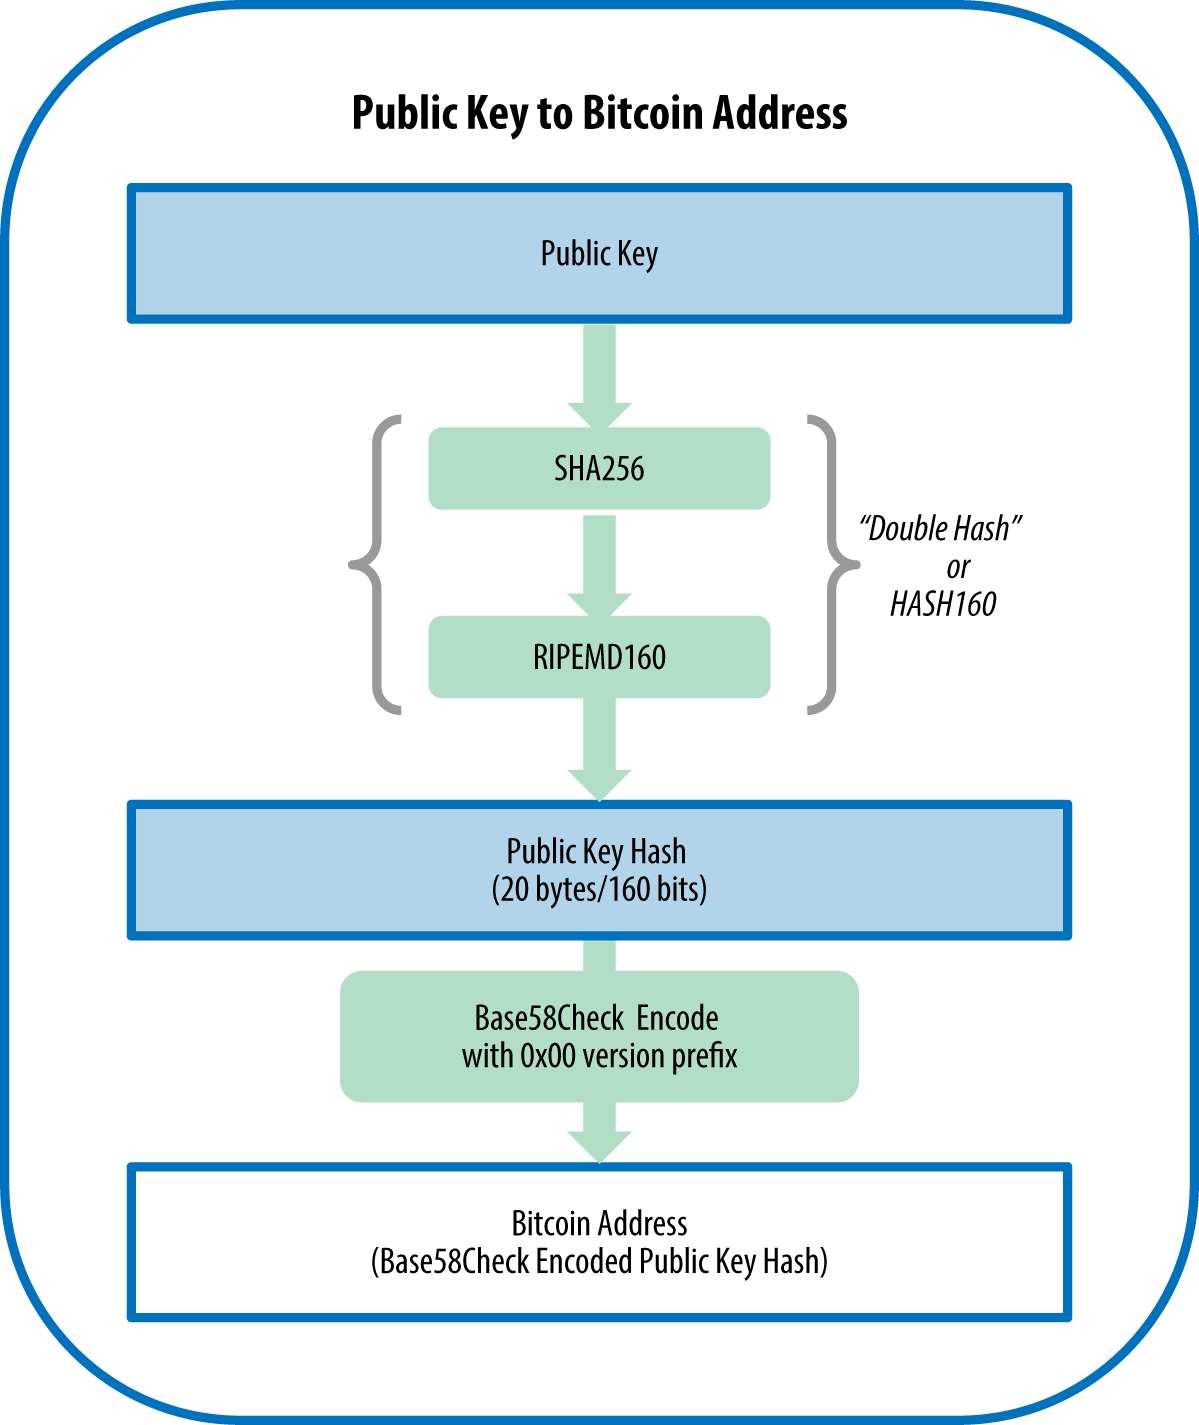
\includegraphics[scale=0.5]{mbc2_0405.png}
\end{frame}



\section{Transaction}
\begin{frame}

\end{frame}



\section{BlockChain}
\begin{frame}
    \frametitle{BlockChain Overview}
    \begin{itemize}
        \item The block chain provides Bitcoin's public ledger, an ordered and timestamped record of transctions.
        \item This system is used to protect against double spending and modification of previous transactions records.
        \item Each full node in the Bitcoin network independently stores a block chain containing only blocks validated by that node.
    \end{itemize}
    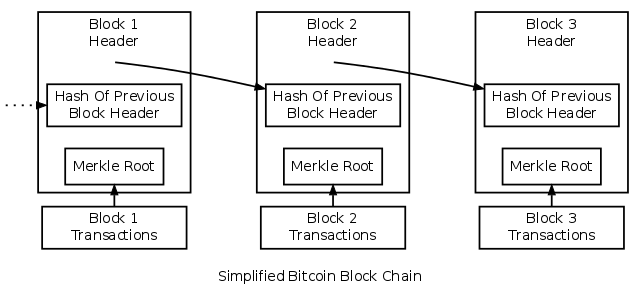
\includegraphics[scale=0.4]{./figures/en-blockchain-overview.png}
\end{frame}

\begin{frame}[fragile]
    \frametitle{BlockChain Data Structure}
    \begin{columns}
        \begin{column}{0.6\textwidth}
            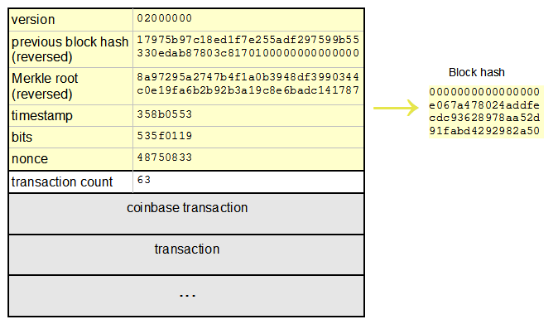
\includegraphics[scale=0.5]{./figures/blockchain-data-structure.png}
        \end{column}
        \begin{column}{0.4\textwidth}
            \includegraphics[scale=0.4]{./figures/mbc2_0902.png}
        \end{column}
    \end{columns}
    \begin{itemize}
        \item \textbf{Block Header}: 80 bytes, whereas transctions is at least 250 bytes.
        \item \textbf{Nonce}: A counter used for proof-of-work algorithm.
        \item \textbf{Difficulty}: How difficult it is to find a hash below a given target.
        \item \textbf{Coinbase}: The content of the \alert{input} of a generation transction.
    \end{itemize}
    \begin{lstlisting}[language=Python]
The Times 03/Jan/2009 Chancellor on brink of second bailout for banks. \end{lstlisting}
\end{frame}

\begin{frame}[fragile]
    \frametitle{The Genesis Block}
    \begin{lstlisting}[language=Python]
bitcoind getblock 000000000019d6689c085ae165831e934ff763ae46a2a6c172b3f1b60a8ce26f
{
    "hash" : "000000000019d6689c085ae165831e934ff763ae46a2a6c172b3f1b60a8ce26f",
    "confirmations" : 308321,
    "size" : 285,
    "height" : 0,
    "version" : 1,
    "merkleroot" : "4a5e1e4baab89f3a32518a88c31bc87f618f76673e2cc77ab2127b7afdeda33b",
    "tx" : [
        "4a5e1e4baab89f3a32518a88c31bc87f618f76673e2cc77ab2127b7afdeda33b"
    ],
    "time" : 1231006505,
    "nonce" : 2083236893,
    "bits" : "1d00ffff",
    "difficulty" : 1.00000000,
    "nextblockhash" : "00000000839a8e6886ab5951d76f411475428afc90947ee320161bbf18eb6048"
}
    \end{lstlisting}
    The difficulty value updates every 2 weeks to ensure that it takes 10 minutes(on average) to add a new block to the BlockChain.
    \begin{lstlisting}[language=Python]
0x00ffff * 2**(8*(0x1d-3))=0x00000000FFFF0000000000000000000000000000000000000000000000000000 \end{lstlisting}
\end{frame}

\begin{frame}[fragile]
    \frametitle{Proof Of Work}
    \begin{itemize}
        \item Block contains transctions to be validated and previous hash value.
        \item Pick a nonce such that \textbf{H(prev hash, nonce, Tx) < E}.
        \item Verification is easy, But proof-of-work is hard.
    \end{itemize}
    \includegraphics[scale=0.5]{./figures/block-puzzle.png}
\end{frame}

\begin{frame}[fragile]
    \frametitle{Difficulty Target and Re-Target}
    Every 2016 blocks, all node re-target the Proof-of-Work difficulty.
    \begin{lstlisting}[language=Python]
New Difficulty = Old Difficulty * (20160 minutes / Actual Time of Last 2016 Blocks)
The Target = The maximum target / current difficulty.
The maximum target is:
    0x00000000FFFF0000000000000000000000000000000000000000000000000000 \end{lstlisting}

    Re-Target Code in bitcoind
    \begin{lstlisting}[language=C++]
    // Limit adjustment step
    int64_t nActualTimespan = pindexLast->GetBlockTime() - nFirstBlockTime;
    LogPrintf("  nActualTimespan = %d  before bounds\n", nActualTimespan);
    if (nActualTimespan < params.nPowTargetTimespan/4)
        nActualTimespan = params.nPowTargetTimespan/4;
    if (nActualTimespan > params.nPowTargetTimespan*4)
        nActualTimespan = params.nPowTargetTimespan*4;

    // Retarget
    const arith_uint256 bnPowLimit = UintToArith256(params.powLimit);
    arith_uint256 bnNew;
    arith_uint256 bnOld;
    bnNew.SetCompact(pindexLast->nBits);
    bnOld = bnNew;
    bnNew *= nActualTimespan;
    bnNew /= params.nPowTargetTimespan;

    if (bnNew > bnPowLimit)
        bnNew = bnPowLimit; \end{lstlisting}
\end{frame}



\section{Mining}
\begin{frame}
    \frametitle{Mining and Consensus}
    \begin{block}{Definition}
        Mining \alert{secures} the bitcoin system and enables the emergence of network-wide \alert{consensus} without a \alert{central authority}. The reward of newly mined coins and transaction fees is an \alert{incentive scheme} that aligns the actions of miners with the \alert{security of the network}, while simultaneously implementing the \alert{monetary supply}.
    \end{block}
    \begin{figure}[htbp]
        \subfigure{
        \begin{minipage}[b]{0.45\textwidth}
            \centering
            \includegraphics[scale=0.2]{mining-reward.png}
        \end{minipage}
    }
        \subfigure{
        \begin{minipage}[b]{0.45\textwidth}
            \centering
            \includegraphics[scale=0.6]{mbc2_1001.png}
        \end{minipage}
    }
    \end{figure}
\end{frame}

\begin{frame}
    \frametitle{Decentralize Consensus}
    When there is no central authority, how can everyone in the network realize consensus?
    \begin{itemize}
        \item \textbf{tradition consensus algorithm}
            \begin{itemize}
                \item Paxos, Raft, \ldots
                \item Failure model: Not Byzantine(Node may fail, But not malicious)
                \item Leader election.
                \item Focusing on log(database), more universe
            \end{itemize}
        \item \textbf{blockchain consensus algorithm}
            \begin{itemize}
                \item PoW, PoS(Proof of Stake), \ldots
                \item Failure model: Byzantine(Node may be malicious)
                \item No election.
                \item Focusing on transaction.
            \end{itemize}
    \end{itemize}
    Anyway, all the consensus algorithm comply with the \alert{majority rule}.
\end{frame}

\begin{frame}
    \frametitle{Byzantine Generals' Problem}
    Story background:
    \begin{itemize}
        \item Generals of army surround enemy city
        \item Actions in union required to win
        \item Some generals may be traitors
        \item Messengers are reliable
    \end{itemize}
    \begin{center}
        \includegraphics[scale=0.15]{byzantine-generals-problem.png}
    \end{center}
%    Results:
%    \begin{itemize}
%        \item No solution exists if less than or equal to 2/3 generals are loyal.
%    \end{itemize}
\end{frame}

\begin{frame}
    \frametitle{Proof of Work}
    \begin{itemize}
        \item \textbf{Fork}
            \begin{itemize}
                \item when 2 miners mine a block at the same time.
            \end{itemize}
        \item \textbf{Orphan}
            \begin{itemize}
                \item Only one can be in the chain, the other is called \alert{Orphan}
            \end{itemize}
        \item \textbf{Fork/Dispute Resolution}
            \begin{itemize}
                \item The longest block chain is valid.
            \end{itemize}
    \end{itemize}
    \begin{center}
        \includegraphics[scale=0.5]{mbc2_1009.png}
    \end{center}
\end{frame}

\begin{frame}
    \frametitle{Block Chain Fork}
    \includegraphics[scale=0.7]{mbc2_1002.png}
\end{frame}

\begin{frame}
    \frametitle{Block Chain Fork}
    \includegraphics[scale=0.5]{mbc2_1003.png}
\end{frame}

\begin{frame}
    \frametitle{Block Chain Fork}
    \includegraphics[scale=0.5]{mbc2_1004.png}
\end{frame}

\begin{frame}
    \frametitle{Block Chain Fork}
    \includegraphics[scale=0.5]{mbc2_1005.png}
\end{frame}

\begin{frame}
    \frametitle{Block Chain Fork}
    \includegraphics[scale=0.5]{mbc2_1006.png}
\end{frame}

\begin{frame}
    \frametitle{Double Spending Attack}
    Any attacker is competing against the whole network.
    \begin{center}
        \includegraphics[scale=0.16]{double-spending.png}
    \end{center}
    \begin{itemize}
        \item Each block contains a reference to the previous block.
        \item 51\% computing power of the whole network have a 50\% chance to solve a block before some other node does.
        \item Create 2, 3 or more blocks in a row is even harder.
    \end{itemize}
\end{frame}

\begin{frame}
    \frametitle{Blockchain Transactions Security}
    Transactions get more and more secure with time.
    \begin{itemize}
        \item A block is add to the chain every 10 minutes on average.
        \item Waiting for 6 block(1 hour) gives a quite high probability that the transaction has been processed and is \alert{non reversible}.
    \end{itemize}
    \includegraphics[scale=0.2]{bitcoin-security.png}
\end{frame}

\begin{frame}
    \frametitle{Two Generals' Problem}
    \includegraphics[scale=0.5]{two-generals-problem.png}
    \begin{itemize}
        \item \alert{Two generals} need to coordinate an attack.
            \begin{itemize}
                \item Must \alert{agree} on time to attack.
                \item They will win only if they attack \alert{simultaneously}.
                \item Communicate through \alert{messengers}.
                \item Messengers may be \alert{killed} on their way.
            \end{itemize}
    \end{itemize}
\end{frame}

\begin{frame}
    \frametitle{Two Generals' Problem}
    \includegraphics[scale=0.5]{two-generals-problem.png}
    \begin{itemize}
        \item Let's try to solve it for general g1 and g2.
        \item g1 sends \alert{time of attack} to g2.
            \begin{itemize}
                \item \alert{Problem}: how to ensure g2 received message?
                \item \alert{Solution}: let g2 ack receipt of message.
                \item \alert{Problem}: how to ensure g1 received ack?
                \item \alert{Solution}: let g1 ack the receipt of the ack.
                \item \ldots
            \end{itemize}
        \item This problem is \alert{impossible} to solve!
    \end{itemize}
\end{frame}

\begin{frame}
    \frametitle{Engineering approaches: TCP handshake}
    A progmatic approach to dealing with the Two Generals's Problem
    \begin{itemize}
        \item Accept the \alert{uncertainty} of the Communication channel.
        \item Not attempt to eliminate it, but mitigate it to an acceptable degree.
        \item Classic Example is TCP handshake protocol.
    \end{itemize}
    \includegraphics[scale=0.4]{tcp-handshake.png}
\end{frame}


\end{document}
